\documentclass[11pt]{article}

\usepackage[english]{babel}
\usepackage[T1]{fontenc}
\usepackage[utf8]{inputenc}
%\usepackage{mathptm}
%\usepackage{times}
\usepackage{amsmath}
\usepackage{amsthm}
\usepackage{mathtools}
\usepackage{listings}
\usepackage{tikz}
\usepackage{subcaption}
\usepackage{rotating}

\usetikzlibrary{calc}
\usetikzlibrary{patterns}

\frenchspacing

\lstset{
  basicstyle = \ttfamily
}

\DeclarePairedDelimiter{\ceil}{\lceil}{\rceil}
\DeclarePairedDelimiter{\floor}{\lfloor}{\rfloor}

\newcommand{\define}{\stackrel{\mathit{def}}=}
\newcommand{\pleft}{\mathit{left}}
\newcommand{\pright}{\mathit{right}}
\newcommand{\depth}{\mathit{depth}}
\newcommand{\val}{\mathit{val}}
\newcommand{\LF}{\mathit{LF}}

%\centering in all figures
\makeatletter
\g@addto@macro\@floatboxreset\centering
\makeatother

\newtheorem{lemma}{Lemma}

%listings for Haskell / FP
\lstloadlanguages{Haskell}
\lstnewenvironment{code}
{
  \lstset{
  %language=Haskell
  }
  \csname lst@SetFirstLabel\endcsname
}
{
  \csname lst@SaveFirstLabel\endcsname
}
\lstset{
  language=Haskell,
  basicstyle=\small\ttfamily,
  flexiblecolumns=false,
  basewidth={0.5em,0.45em},
  literate={+}{{$+$}}1 {/}{{$/$}}1 {*}{{$*$}}1 {=}{{$=$}}1
           {>}{{$>$}}1 {<}{{$<$}}1 {\\}{{$\lambda$}}1
           {\\\\}{{\char`\\\char`\\}}1
           {->}{{$\rightarrow$}}2
           {>=}{{$\geq$}}2 {<-}{{$\leftarrow$}}2
           {<=}{{$\leq$}}2 {=>}{{$\Rightarrow$}}2
           {\ .}{{$\circ$}}2 {\ .\ }{{$\circ$}}3
           {>>}{{>>}}2 {>>=}{{>>=}}2
           {|}{{$\mid$}}1
           {==}{{$==$}}2
           {++}{{$++$}}2
           % Network specific
           {|>}{{$\triangleright$}}2
}

\newcommand{\lst}{\lstinline}
\newcommand{\ignore}[1]{}

\begin{document}

\title{A minimum depth prefix network (that is far from optimal)}

\author{Li-yao Xia}% {firstname}.{lastname}@ens.fr

\maketitle

\input{../PNet.lhs}
\input{Construct.lhs}

\newpage

\begin{table}
  \begin{tabular}{| r || r | r | r |}
    \hline
    Depth &      C & Ladner-Fischer & Minimum \\
    \hline
        3 &     12 &             12 &      12 \\
        4 &     31 &             31 &      31 \\
        5 &     74 &             74 &      74 \\
        6 &    168 &            168 &     167 \\
        7 &    369 &            369 &     364 \\
        8 &    793 &            792 &     773 \\
        9 &   1679 &           1672 &    1614 \\
       10 &   3518 &           3487 &    3327 \\
       11 &   7315 &           7206 &    6800 \\
       12 &  15122 &          14788 &   13809 \\
       13 &  31120 &          30185 &   27922 \\
       14 &  63814 &          61356 &   56275 \\
       15 & 130481 &         124308 &  113172 \\
       16 & 266176 &         251199 &  227221 \\
       17 & 541953 &         506578 &  455702 \\
       18 &      - &        1019920 &  913175 \\
       19 &      - &        2050785 & 1828888 \\
       20 &      - &        4119280 & 3661337 \\
    \hline              
  \end{tabular}         
  \caption{More values could be computed in the first column using memoization
  and other optimizations.}
\end{table}


\begin{figure}
  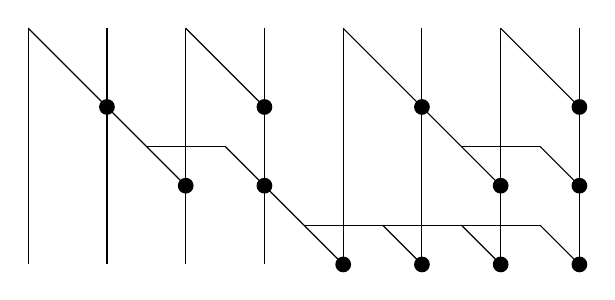
\begin{tikzpicture}\begin{scope}[scale=1.00000]\path[draw] (0.00000,0.00000) -- (0.00000,3.00000) ; \path[draw] (1.00000,0.00000) -- (1.00000,3.00000) ; \path[draw] (2.00000,0.00000) -- (2.00000,3.00000) ; \path[draw] (3.00000,0.00000) -- (3.00000,3.00000) ; \path[draw] (4.00000,0.00000) -- (4.00000,3.00000) ; \path[draw] (5.00000,0.00000) -- (5.00000,3.00000) ; \path[draw] (6.00000,0.00000) -- (6.00000,3.00000) ; \path[draw] (7.00000,0.00000) -- (7.00000,3.00000) ; \path[draw] (3.00000,1.00000) -- (3.50000,0.50000) ; \path[draw] (3.50000,0.50000) -- (6.50000,0.50000) ; \path[draw] (3.50000,0.50000) -- (4.00000,0.00000) ; \path[draw] (4.50000,0.50000) -- (5.00000,0.00000) ; \path[draw] (5.50000,0.50000) -- (6.00000,0.00000) ; \path[draw] (6.50000,0.50000) -- (7.00000,0.00000) ; \path[fill] (4.00000,0.00000) circle (0.10000) ; \path[fill] (5.00000,0.00000) circle (0.10000) ; \path[fill] (6.00000,0.00000) circle (0.10000) ; \path[fill] (7.00000,0.00000) circle (0.10000) ; \path[draw] (1.00000,2.00000) -- (1.50000,1.50000) ; \path[draw] (1.50000,1.50000) -- (2.50000,1.50000) ; \path[draw] (1.50000,1.50000) -- (2.00000,1.00000) ; \path[draw] (2.50000,1.50000) -- (3.00000,1.00000) ; \path[fill] (2.00000,1.00000) circle (0.10000) ; \path[fill] (3.00000,1.00000) circle (0.10000) ; \path[draw] (5.00000,2.00000) -- (5.50000,1.50000) ; \path[draw] (5.50000,1.50000) -- (6.50000,1.50000) ; \path[draw] (5.50000,1.50000) -- (6.00000,1.00000) ; \path[draw] (6.50000,1.50000) -- (7.00000,1.00000) ; \path[fill] (6.00000,1.00000) circle (0.10000) ; \path[fill] (7.00000,1.00000) circle (0.10000) ; \path[draw] (0.00000,3.00000) -- (0.50000,2.50000) ; \path[draw] (0.50000,2.50000) -- (1.00000,2.00000) ; \path[fill] (1.00000,2.00000) circle (0.10000) ; \path[draw] (2.00000,3.00000) -- (2.50000,2.50000) ; \path[draw] (2.50000,2.50000) -- (3.00000,2.00000) ; \path[fill] (3.00000,2.00000) circle (0.10000) ; \path[draw] (4.00000,3.00000) -- (4.50000,2.50000) ; \path[draw] (4.50000,2.50000) -- (5.00000,2.00000) ; \path[fill] (5.00000,2.00000) circle (0.10000) ; \path[draw] (6.00000,3.00000) -- (6.50000,2.50000) ; \path[draw] (6.50000,2.50000) -- (7.00000,2.00000) ; \path[fill] (7.00000,2.00000) circle (0.10000) ; \end{scope}\end{tikzpicture}
  \caption{$n=8$}
\end{figure}

\begin{figure}
  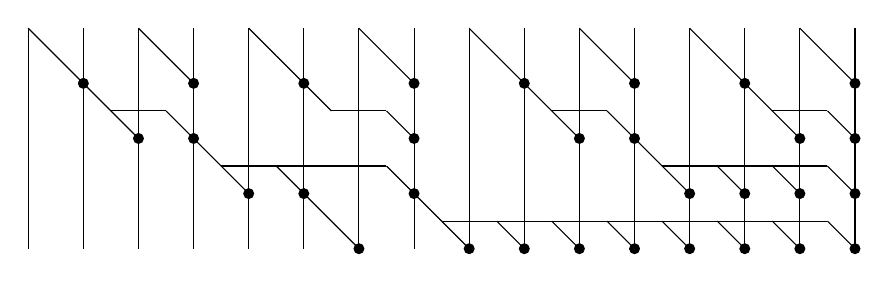
\begin{tikzpicture}
\begin{scope}[scale=0.70000]
\path[draw] (0.00000,0.00000) -- (0.00000,4.00000) ; 
\path[draw] (1.00000,0.00000) -- (1.00000,4.00000) ; 
\path[draw] (2.00000,0.00000) -- (2.00000,4.00000) ; 
\path[draw] (3.00000,0.00000) -- (3.00000,4.00000) ; 
\path[draw] (4.00000,0.00000) -- (4.00000,4.00000) ; 
\path[draw] (5.00000,0.00000) -- (5.00000,4.00000) ; 
\path[draw] (6.00000,0.00000) -- (6.00000,4.00000) ; 
\path[draw] (7.00000,0.00000) -- (7.00000,4.00000) ; 
\path[draw] (8.00000,0.00000) -- (8.00000,4.00000) ; 
\path[draw] (9.00000,0.00000) -- (9.00000,4.00000) ; 
\path[draw] (10.00000,0.00000) -- (10.00000,4.00000) ; 
\path[draw] (11.00000,0.00000) -- (11.00000,4.00000) ; 
\path[draw] (12.00000,0.00000) -- (12.00000,4.00000) ; 
\path[draw] (13.00000,0.00000) -- (13.00000,4.00000) ; 
\path[draw] (14.00000,0.00000) -- (14.00000,4.00000) ; 
\path[draw] (15.00000,0.00000) -- (15.00000,4.00000) ; 
\path[draw] (5.00000,1.00000) -- (5.50000,0.50000) ; 
\path[draw] (5.50000,0.50000) -- (6.00000,0.00000) ; 
\path[fill] (6.00000,0.00000) circle (0.10000) ; 
\path[draw] (7.00000,1.00000) -- (7.50000,0.50000) ; 
\path[draw] (7.50000,0.50000) -- (14.50000,0.50000) ; 
\path[draw] (7.50000,0.50000) -- (8.00000,0.00000) ; 
\path[draw] (8.50000,0.50000) -- (9.00000,0.00000) ; 
\path[draw] (9.50000,0.50000) -- (10.00000,0.00000) ; 
\path[draw] (10.50000,0.50000) -- (11.00000,0.00000) ; 
\path[draw] (11.50000,0.50000) -- (12.00000,0.00000) ; 
\path[draw] (12.50000,0.50000) -- (13.00000,0.00000) ; 
\path[draw] (13.50000,0.50000) -- (14.00000,0.00000) ; 
\path[draw] (14.50000,0.50000) -- (15.00000,0.00000) ; 
\path[fill] (8.00000,0.00000) circle (0.10000) ; 
\path[fill] (9.00000,0.00000) circle (0.10000) ; 
\path[fill] (10.00000,0.00000) circle (0.10000) ; 
\path[fill] (11.00000,0.00000) circle (0.10000) ; 
\path[fill] (12.00000,0.00000) circle (0.10000) ; 
\path[fill] (13.00000,0.00000) circle (0.10000) ; 
\path[fill] (14.00000,0.00000) circle (0.10000) ; 
\path[fill] (15.00000,0.00000) circle (0.10000) ; 
\path[draw] (3.00000,2.00000) -- (3.50000,1.50000) ; 
\path[draw] (3.50000,1.50000) -- (6.50000,1.50000) ; 
\path[draw] (3.50000,1.50000) -- (4.00000,1.00000) ; 
\path[draw] (4.50000,1.50000) -- (5.00000,1.00000) ; 
\path[draw] (6.50000,1.50000) -- (7.00000,1.00000) ; 
\path[fill] (4.00000,1.00000) circle (0.10000) ; 
\path[fill] (5.00000,1.00000) circle (0.10000) ; 
\path[fill] (7.00000,1.00000) circle (0.10000) ; 
\path[draw] (11.00000,2.00000) -- (11.50000,1.50000) ; 
\path[draw] (11.50000,1.50000) -- (14.50000,1.50000) ; 
\path[draw] (11.50000,1.50000) -- (12.00000,1.00000) ; 
\path[draw] (12.50000,1.50000) -- (13.00000,1.00000) ; 
\path[draw] (13.50000,1.50000) -- (14.00000,1.00000) ; 
\path[draw] (14.50000,1.50000) -- (15.00000,1.00000) ; 
\path[fill] (12.00000,1.00000) circle (0.10000) ; 
\path[fill] (13.00000,1.00000) circle (0.10000) ; 
\path[fill] (14.00000,1.00000) circle (0.10000) ; 
\path[fill] (15.00000,1.00000) circle (0.10000) ; 
\path[draw] (1.00000,3.00000) -- (1.50000,2.50000) ; 
\path[draw] (1.50000,2.50000) -- (2.50000,2.50000) ; 
\path[draw] (1.50000,2.50000) -- (2.00000,2.00000) ; 
\path[draw] (2.50000,2.50000) -- (3.00000,2.00000) ; 
\path[fill] (2.00000,2.00000) circle (0.10000) ; 
\path[fill] (3.00000,2.00000) circle (0.10000) ; 
\path[draw] (5.00000,3.00000) -- (5.50000,2.50000) ; 
\path[draw] (5.50000,2.50000) -- (6.50000,2.50000) ; 
\path[draw] (6.50000,2.50000) -- (7.00000,2.00000) ; 
\path[fill] (7.00000,2.00000) circle (0.10000) ; 
\path[draw] (9.00000,3.00000) -- (9.50000,2.50000) ; 
\path[draw] (9.50000,2.50000) -- (10.50000,2.50000) ; 
\path[draw] (9.50000,2.50000) -- (10.00000,2.00000) ; 
\path[draw] (10.50000,2.50000) -- (11.00000,2.00000) ; 
\path[fill] (10.00000,2.00000) circle (0.10000) ; 
\path[fill] (11.00000,2.00000) circle (0.10000) ; 
\path[draw] (13.00000,3.00000) -- (13.50000,2.50000) ; 
\path[draw] (13.50000,2.50000) -- (14.50000,2.50000) ; 
\path[draw] (13.50000,2.50000) -- (14.00000,2.00000) ; 
\path[draw] (14.50000,2.50000) -- (15.00000,2.00000) ; 
\path[fill] (14.00000,2.00000) circle (0.10000) ; 
\path[fill] (15.00000,2.00000) circle (0.10000) ; 
\path[draw] (0.00000,4.00000) -- (0.50000,3.50000) ; 
\path[draw] (0.50000,3.50000) -- (1.00000,3.00000) ; 
\path[fill] (1.00000,3.00000) circle (0.10000) ; 
\path[draw] (2.00000,4.00000) -- (2.50000,3.50000) ; 
\path[draw] (2.50000,3.50000) -- (3.00000,3.00000) ; 
\path[fill] (3.00000,3.00000) circle (0.10000) ; 
\path[draw] (4.00000,4.00000) -- (4.50000,3.50000) ; 
\path[draw] (4.50000,3.50000) -- (5.00000,3.00000) ; 
\path[fill] (5.00000,3.00000) circle (0.10000) ; 
\path[draw] (6.00000,4.00000) -- (6.50000,3.50000) ; 
\path[draw] (6.50000,3.50000) -- (7.00000,3.00000) ; 
\path[fill] (7.00000,3.00000) circle (0.10000) ; 
\path[draw] (8.00000,4.00000) -- (8.50000,3.50000) ; 
\path[draw] (8.50000,3.50000) -- (9.00000,3.00000) ; 
\path[fill] (9.00000,3.00000) circle (0.10000) ; 
\path[draw] (10.00000,4.00000) -- (10.50000,3.50000) ; 
\path[draw] (10.50000,3.50000) -- (11.00000,3.00000) ; 
\path[fill] (11.00000,3.00000) circle (0.10000) ; 
\path[draw] (12.00000,4.00000) -- (12.50000,3.50000) ; 
\path[draw] (12.50000,3.50000) -- (13.00000,3.00000) ; 
\path[fill] (13.00000,3.00000) circle (0.10000) ; 
\path[draw] (14.00000,4.00000) -- (14.50000,3.50000) ; 
\path[draw] (14.50000,3.50000) -- (15.00000,3.00000) ; 
\path[fill] (15.00000,3.00000) circle (0.10000) ; 
\end{scope}
\end{tikzpicture}

  \caption{$n=16$}
\end{figure}

\begin{figure}
  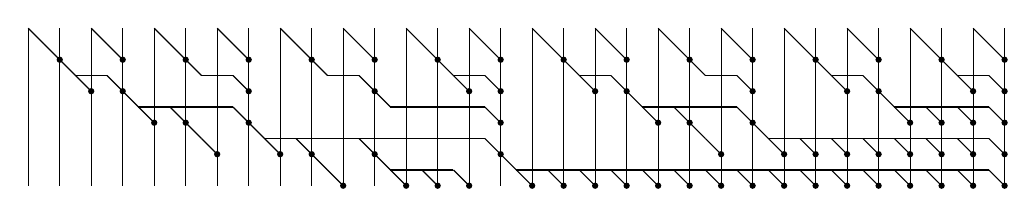
\begin{tikzpicture}
\begin{scope}[scale=0.4000]
\path[draw] (0.00000,0.00000) -- (0.00000,5.00000) ; 
\path[draw] (1.00000,0.00000) -- (1.00000,5.00000) ; 
\path[draw] (2.00000,0.00000) -- (2.00000,5.00000) ; 
\path[draw] (3.00000,0.00000) -- (3.00000,5.00000) ; 
\path[draw] (4.00000,0.00000) -- (4.00000,5.00000) ; 
\path[draw] (5.00000,0.00000) -- (5.00000,5.00000) ; 
\path[draw] (6.00000,0.00000) -- (6.00000,5.00000) ; 
\path[draw] (7.00000,0.00000) -- (7.00000,5.00000) ; 
\path[draw] (8.00000,0.00000) -- (8.00000,5.00000) ; 
\path[draw] (9.00000,0.00000) -- (9.00000,5.00000) ; 
\path[draw] (10.00000,0.00000) -- (10.00000,5.00000) ; 
\path[draw] (11.00000,0.00000) -- (11.00000,5.00000) ; 
\path[draw] (12.00000,0.00000) -- (12.00000,5.00000) ; 
\path[draw] (13.00000,0.00000) -- (13.00000,5.00000) ; 
\path[draw] (14.00000,0.00000) -- (14.00000,5.00000) ; 
\path[draw] (15.00000,0.00000) -- (15.00000,5.00000) ; 
\path[draw] (16.00000,0.00000) -- (16.00000,5.00000) ; 
\path[draw] (17.00000,0.00000) -- (17.00000,5.00000) ; 
\path[draw] (18.00000,0.00000) -- (18.00000,5.00000) ; 
\path[draw] (19.00000,0.00000) -- (19.00000,5.00000) ; 
\path[draw] (20.00000,0.00000) -- (20.00000,5.00000) ; 
\path[draw] (21.00000,0.00000) -- (21.00000,5.00000) ; 
\path[draw] (22.00000,0.00000) -- (22.00000,5.00000) ; 
\path[draw] (23.00000,0.00000) -- (23.00000,5.00000) ; 
\path[draw] (24.00000,0.00000) -- (24.00000,5.00000) ; 
\path[draw] (25.00000,0.00000) -- (25.00000,5.00000) ; 
\path[draw] (26.00000,0.00000) -- (26.00000,5.00000) ; 
\path[draw] (27.00000,0.00000) -- (27.00000,5.00000) ; 
\path[draw] (28.00000,0.00000) -- (28.00000,5.00000) ; 
\path[draw] (29.00000,0.00000) -- (29.00000,5.00000) ; 
\path[draw] (30.00000,0.00000) -- (30.00000,5.00000) ; 
\path[draw] (31.00000,0.00000) -- (31.00000,5.00000) ; 
\path[draw] (9.00000,1.00000) -- (9.50000,0.50000) ; 
\path[draw] (9.50000,0.50000) -- (10.00000,0.00000) ; 
\path[fill] (10.00000,0.00000) circle (0.10000) ; 
\path[draw] (11.00000,1.00000) -- (11.50000,0.50000) ; 
\path[draw] (11.50000,0.50000) -- (13.50000,0.50000) ; 
\path[draw] (11.50000,0.50000) -- (12.00000,0.00000) ; 
\path[draw] (12.50000,0.50000) -- (13.00000,0.00000) ; 
\path[draw] (13.50000,0.50000) -- (14.00000,0.00000) ; 
\path[fill] (12.00000,0.00000) circle (0.10000) ; 
\path[fill] (13.00000,0.00000) circle (0.10000) ; 
\path[fill] (14.00000,0.00000) circle (0.10000) ; 
\path[draw] (15.00000,1.00000) -- (15.50000,0.50000) ; 
\path[draw] (15.50000,0.50000) -- (30.50000,0.50000) ; 
\path[draw] (15.50000,0.50000) -- (16.00000,0.00000) ; 
\path[draw] (16.50000,0.50000) -- (17.00000,0.00000) ; 
\path[draw] (17.50000,0.50000) -- (18.00000,0.00000) ; 
\path[draw] (18.50000,0.50000) -- (19.00000,0.00000) ; 
\path[draw] (19.50000,0.50000) -- (20.00000,0.00000) ; 
\path[draw] (20.50000,0.50000) -- (21.00000,0.00000) ; 
\path[draw] (21.50000,0.50000) -- (22.00000,0.00000) ; 
\path[draw] (22.50000,0.50000) -- (23.00000,0.00000) ; 
\path[draw] (23.50000,0.50000) -- (24.00000,0.00000) ; 
\path[draw] (24.50000,0.50000) -- (25.00000,0.00000) ; 
\path[draw] (25.50000,0.50000) -- (26.00000,0.00000) ; 
\path[draw] (26.50000,0.50000) -- (27.00000,0.00000) ; 
\path[draw] (27.50000,0.50000) -- (28.00000,0.00000) ; 
\path[draw] (28.50000,0.50000) -- (29.00000,0.00000) ; 
\path[draw] (29.50000,0.50000) -- (30.00000,0.00000) ; 
\path[draw] (30.50000,0.50000) -- (31.00000,0.00000) ; 
\path[fill] (16.00000,0.00000) circle (0.10000) ; 
\path[fill] (17.00000,0.00000) circle (0.10000) ; 
\path[fill] (18.00000,0.00000) circle (0.10000) ; 
\path[fill] (19.00000,0.00000) circle (0.10000) ; 
\path[fill] (20.00000,0.00000) circle (0.10000) ; 
\path[fill] (21.00000,0.00000) circle (0.10000) ; 
\path[fill] (22.00000,0.00000) circle (0.10000) ; 
\path[fill] (23.00000,0.00000) circle (0.10000) ; 
\path[fill] (24.00000,0.00000) circle (0.10000) ; 
\path[fill] (25.00000,0.00000) circle (0.10000) ; 
\path[fill] (26.00000,0.00000) circle (0.10000) ; 
\path[fill] (27.00000,0.00000) circle (0.10000) ; 
\path[fill] (28.00000,0.00000) circle (0.10000) ; 
\path[fill] (29.00000,0.00000) circle (0.10000) ; 
\path[fill] (30.00000,0.00000) circle (0.10000) ; 
\path[fill] (31.00000,0.00000) circle (0.10000) ; 
\path[draw] (5.00000,2.00000) -- (5.50000,1.50000) ; 
\path[draw] (5.50000,1.50000) -- (6.00000,1.00000) ; 
\path[fill] (6.00000,1.00000) circle (0.10000) ; 
\path[draw] (7.00000,2.00000) -- (7.50000,1.50000) ; 
\path[draw] (7.50000,1.50000) -- (14.50000,1.50000) ; 
\path[draw] (7.50000,1.50000) -- (8.00000,1.00000) ; 
\path[draw] (8.50000,1.50000) -- (9.00000,1.00000) ; 
\path[draw] (10.50000,1.50000) -- (11.00000,1.00000) ; 
\path[draw] (14.50000,1.50000) -- (15.00000,1.00000) ; 
\path[fill] (8.00000,1.00000) circle (0.10000) ; 
\path[fill] (9.00000,1.00000) circle (0.10000) ; 
\path[fill] (11.00000,1.00000) circle (0.10000) ; 
\path[fill] (15.00000,1.00000) circle (0.10000) ; 
\path[draw] (21.00000,2.00000) -- (21.50000,1.50000) ; 
\path[draw] (21.50000,1.50000) -- (22.00000,1.00000) ; 
\path[fill] (22.00000,1.00000) circle (0.10000) ; 
\path[draw] (23.00000,2.00000) -- (23.50000,1.50000) ; 
\path[draw] (23.50000,1.50000) -- (30.50000,1.50000) ; 
\path[draw] (23.50000,1.50000) -- (24.00000,1.00000) ; 
\path[draw] (24.50000,1.50000) -- (25.00000,1.00000) ; 
\path[draw] (25.50000,1.50000) -- (26.00000,1.00000) ; 
\path[draw] (26.50000,1.50000) -- (27.00000,1.00000) ; 
\path[draw] (27.50000,1.50000) -- (28.00000,1.00000) ; 
\path[draw] (28.50000,1.50000) -- (29.00000,1.00000) ; 
\path[draw] (29.50000,1.50000) -- (30.00000,1.00000) ; 
\path[draw] (30.50000,1.50000) -- (31.00000,1.00000) ; 
\path[fill] (24.00000,1.00000) circle (0.10000) ; 
\path[fill] (25.00000,1.00000) circle (0.10000) ; 
\path[fill] (26.00000,1.00000) circle (0.10000) ; 
\path[fill] (27.00000,1.00000) circle (0.10000) ; 
\path[fill] (28.00000,1.00000) circle (0.10000) ; 
\path[fill] (29.00000,1.00000) circle (0.10000) ; 
\path[fill] (30.00000,1.00000) circle (0.10000) ; 
\path[fill] (31.00000,1.00000) circle (0.10000) ; 
\path[draw] (3.00000,3.00000) -- (3.50000,2.50000) ; 
\path[draw] (3.50000,2.50000) -- (6.50000,2.50000) ; 
\path[draw] (3.50000,2.50000) -- (4.00000,2.00000) ; 
\path[draw] (4.50000,2.50000) -- (5.00000,2.00000) ; 
\path[draw] (6.50000,2.50000) -- (7.00000,2.00000) ; 
\path[fill] (4.00000,2.00000) circle (0.10000) ; 
\path[fill] (5.00000,2.00000) circle (0.10000) ; 
\path[fill] (7.00000,2.00000) circle (0.10000) ; 
\path[draw] (11.00000,3.00000) -- (11.50000,2.50000) ; 
\path[draw] (11.50000,2.50000) -- (14.50000,2.50000) ; 
\path[draw] (14.50000,2.50000) -- (15.00000,2.00000) ; 
\path[fill] (15.00000,2.00000) circle (0.10000) ; 
\path[draw] (19.00000,3.00000) -- (19.50000,2.50000) ; 
\path[draw] (19.50000,2.50000) -- (22.50000,2.50000) ; 
\path[draw] (19.50000,2.50000) -- (20.00000,2.00000) ; 
\path[draw] (20.50000,2.50000) -- (21.00000,2.00000) ; 
\path[draw] (22.50000,2.50000) -- (23.00000,2.00000) ; 
\path[fill] (20.00000,2.00000) circle (0.10000) ; 
\path[fill] (21.00000,2.00000) circle (0.10000) ; 
\path[fill] (23.00000,2.00000) circle (0.10000) ; 
\path[draw] (27.00000,3.00000) -- (27.50000,2.50000) ; 
\path[draw] (27.50000,2.50000) -- (30.50000,2.50000) ; 
\path[draw] (27.50000,2.50000) -- (28.00000,2.00000) ; 
\path[draw] (28.50000,2.50000) -- (29.00000,2.00000) ; 
\path[draw] (29.50000,2.50000) -- (30.00000,2.00000) ; 
\path[draw] (30.50000,2.50000) -- (31.00000,2.00000) ; 
\path[fill] (28.00000,2.00000) circle (0.10000) ; 
\path[fill] (29.00000,2.00000) circle (0.10000) ; 
\path[fill] (30.00000,2.00000) circle (0.10000) ; 
\path[fill] (31.00000,2.00000) circle (0.10000) ; 
\path[draw] (1.00000,4.00000) -- (1.50000,3.50000) ; 
\path[draw] (1.50000,3.50000) -- (2.50000,3.50000) ; 
\path[draw] (1.50000,3.50000) -- (2.00000,3.00000) ; 
\path[draw] (2.50000,3.50000) -- (3.00000,3.00000) ; 
\path[fill] (2.00000,3.00000) circle (0.10000) ; 
\path[fill] (3.00000,3.00000) circle (0.10000) ; 
\path[draw] (5.00000,4.00000) -- (5.50000,3.50000) ; 
\path[draw] (5.50000,3.50000) -- (6.50000,3.50000) ; 
\path[draw] (6.50000,3.50000) -- (7.00000,3.00000) ; 
\path[fill] (7.00000,3.00000) circle (0.10000) ; 
\path[draw] (9.00000,4.00000) -- (9.50000,3.50000) ; 
\path[draw] (9.50000,3.50000) -- (10.50000,3.50000) ; 
\path[draw] (10.50000,3.50000) -- (11.00000,3.00000) ; 
\path[fill] (11.00000,3.00000) circle (0.10000) ; 
\path[draw] (13.00000,4.00000) -- (13.50000,3.50000) ; 
\path[draw] (13.50000,3.50000) -- (14.50000,3.50000) ; 
\path[draw] (13.50000,3.50000) -- (14.00000,3.00000) ; 
\path[draw] (14.50000,3.50000) -- (15.00000,3.00000) ; 
\path[fill] (14.00000,3.00000) circle (0.10000) ; 
\path[fill] (15.00000,3.00000) circle (0.10000) ; 
\path[draw] (17.00000,4.00000) -- (17.50000,3.50000) ; 
\path[draw] (17.50000,3.50000) -- (18.50000,3.50000) ; 
\path[draw] (17.50000,3.50000) -- (18.00000,3.00000) ; 
\path[draw] (18.50000,3.50000) -- (19.00000,3.00000) ; 
\path[fill] (18.00000,3.00000) circle (0.10000) ; 
\path[fill] (19.00000,3.00000) circle (0.10000) ; 
\path[draw] (21.00000,4.00000) -- (21.50000,3.50000) ; 
\path[draw] (21.50000,3.50000) -- (22.50000,3.50000) ; 
\path[draw] (22.50000,3.50000) -- (23.00000,3.00000) ; 
\path[fill] (23.00000,3.00000) circle (0.10000) ; 
\path[draw] (25.00000,4.00000) -- (25.50000,3.50000) ; 
\path[draw] (25.50000,3.50000) -- (26.50000,3.50000) ; 
\path[draw] (25.50000,3.50000) -- (26.00000,3.00000) ; 
\path[draw] (26.50000,3.50000) -- (27.00000,3.00000) ; 
\path[fill] (26.00000,3.00000) circle (0.10000) ; 
\path[fill] (27.00000,3.00000) circle (0.10000) ; 
\path[draw] (29.00000,4.00000) -- (29.50000,3.50000) ; 
\path[draw] (29.50000,3.50000) -- (30.50000,3.50000) ; 
\path[draw] (29.50000,3.50000) -- (30.00000,3.00000) ; 
\path[draw] (30.50000,3.50000) -- (31.00000,3.00000) ; 
\path[fill] (30.00000,3.00000) circle (0.10000) ; 
\path[fill] (31.00000,3.00000) circle (0.10000) ; 
\path[draw] (0.00000,5.00000) -- (0.50000,4.50000) ; 
\path[draw] (0.50000,4.50000) -- (1.00000,4.00000) ; 
\path[fill] (1.00000,4.00000) circle (0.10000) ; 
\path[draw] (2.00000,5.00000) -- (2.50000,4.50000) ; 
\path[draw] (2.50000,4.50000) -- (3.00000,4.00000) ; 
\path[fill] (3.00000,4.00000) circle (0.10000) ; 
\path[draw] (4.00000,5.00000) -- (4.50000,4.50000) ; 
\path[draw] (4.50000,4.50000) -- (5.00000,4.00000) ; 
\path[fill] (5.00000,4.00000) circle (0.10000) ; 
\path[draw] (6.00000,5.00000) -- (6.50000,4.50000) ; 
\path[draw] (6.50000,4.50000) -- (7.00000,4.00000) ; 
\path[fill] (7.00000,4.00000) circle (0.10000) ; 
\path[draw] (8.00000,5.00000) -- (8.50000,4.50000) ; 
\path[draw] (8.50000,4.50000) -- (9.00000,4.00000) ; 
\path[fill] (9.00000,4.00000) circle (0.10000) ; 
\path[draw] (10.00000,5.00000) -- (10.50000,4.50000) ; 
\path[draw] (10.50000,4.50000) -- (11.00000,4.00000) ; 
\path[fill] (11.00000,4.00000) circle (0.10000) ; 
\path[draw] (12.00000,5.00000) -- (12.50000,4.50000) ; 
\path[draw] (12.50000,4.50000) -- (13.00000,4.00000) ; 
\path[fill] (13.00000,4.00000) circle (0.10000) ; 
\path[draw] (14.00000,5.00000) -- (14.50000,4.50000) ; 
\path[draw] (14.50000,4.50000) -- (15.00000,4.00000) ; 
\path[fill] (15.00000,4.00000) circle (0.10000) ; 
\path[draw] (16.00000,5.00000) -- (16.50000,4.50000) ; 
\path[draw] (16.50000,4.50000) -- (17.00000,4.00000) ; 
\path[fill] (17.00000,4.00000) circle (0.10000) ; 
\path[draw] (18.00000,5.00000) -- (18.50000,4.50000) ; 
\path[draw] (18.50000,4.50000) -- (19.00000,4.00000) ; 
\path[fill] (19.00000,4.00000) circle (0.10000) ; 
\path[draw] (20.00000,5.00000) -- (20.50000,4.50000) ; 
\path[draw] (20.50000,4.50000) -- (21.00000,4.00000) ; 
\path[fill] (21.00000,4.00000) circle (0.10000) ; 
\path[draw] (22.00000,5.00000) -- (22.50000,4.50000) ; 
\path[draw] (22.50000,4.50000) -- (23.00000,4.00000) ; 
\path[fill] (23.00000,4.00000) circle (0.10000) ; 
\path[draw] (24.00000,5.00000) -- (24.50000,4.50000) ; 
\path[draw] (24.50000,4.50000) -- (25.00000,4.00000) ; 
\path[fill] (25.00000,4.00000) circle (0.10000) ; 
\path[draw] (26.00000,5.00000) -- (26.50000,4.50000) ; 
\path[draw] (26.50000,4.50000) -- (27.00000,4.00000) ; 
\path[fill] (27.00000,4.00000) circle (0.10000) ; 
\path[draw] (28.00000,5.00000) -- (28.50000,4.50000) ; 
\path[draw] (28.50000,4.50000) -- (29.00000,4.00000) ; 
\path[fill] (29.00000,4.00000) circle (0.10000) ; 
\path[draw] (30.00000,5.00000) -- (30.50000,4.50000) ; 
\path[draw] (30.50000,4.50000) -- (31.00000,4.00000) ; 
\path[fill] (31.00000,4.00000) circle (0.10000) ; 
\end{scope}
\end{tikzpicture}

  \caption{$n=32$}
\end{figure}

\begin{sidewaysfigure}
  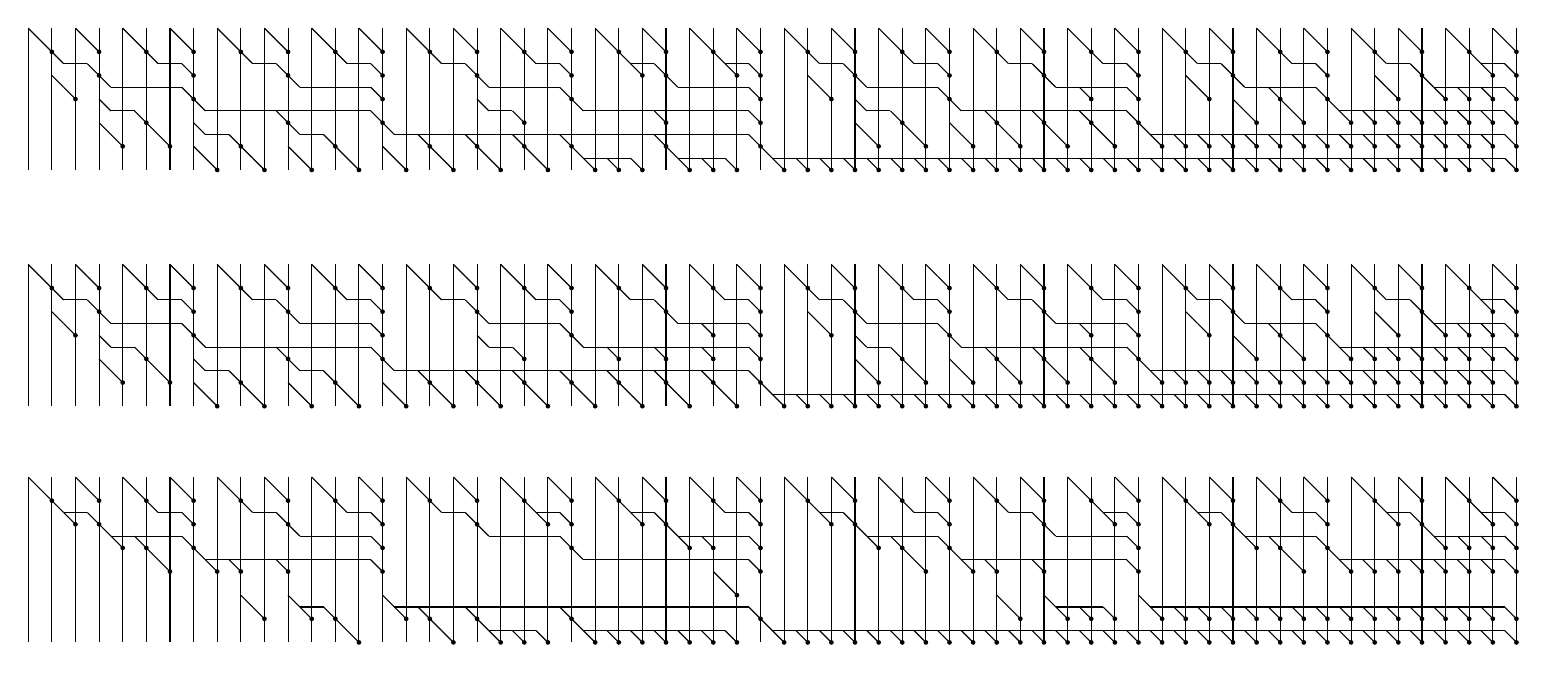
\begin{tikzpicture}
\begin{scope}[scale=0.30000]
\path[draw] (0.00000,0.00000) -- (0.00000,7.00000) ; 
\path[draw] (1.00000,0.00000) -- (1.00000,7.00000) ; 
\path[draw] (2.00000,0.00000) -- (2.00000,7.00000) ; 
\path[draw] (3.00000,0.00000) -- (3.00000,7.00000) ; 
\path[draw] (4.00000,0.00000) -- (4.00000,7.00000) ; 
\path[draw] (5.00000,0.00000) -- (5.00000,7.00000) ; 
\path[draw] (6.00000,0.00000) -- (6.00000,7.00000) ; 
\path[draw] (7.00000,0.00000) -- (7.00000,7.00000) ; 
\path[draw] (8.00000,0.00000) -- (8.00000,7.00000) ; 
\path[draw] (9.00000,0.00000) -- (9.00000,7.00000) ; 
\path[draw] (10.00000,0.00000) -- (10.00000,7.00000) ; 
\path[draw] (11.00000,0.00000) -- (11.00000,7.00000) ; 
\path[draw] (12.00000,0.00000) -- (12.00000,7.00000) ; 
\path[draw] (13.00000,0.00000) -- (13.00000,7.00000) ; 
\path[draw] (14.00000,0.00000) -- (14.00000,7.00000) ; 
\path[draw] (15.00000,0.00000) -- (15.00000,7.00000) ; 
\path[draw] (16.00000,0.00000) -- (16.00000,7.00000) ; 
\path[draw] (17.00000,0.00000) -- (17.00000,7.00000) ; 
\path[draw] (18.00000,0.00000) -- (18.00000,7.00000) ; 
\path[draw] (19.00000,0.00000) -- (19.00000,7.00000) ; 
\path[draw] (20.00000,0.00000) -- (20.00000,7.00000) ; 
\path[draw] (21.00000,0.00000) -- (21.00000,7.00000) ; 
\path[draw] (22.00000,0.00000) -- (22.00000,7.00000) ; 
\path[draw] (23.00000,0.00000) -- (23.00000,7.00000) ; 
\path[draw] (24.00000,0.00000) -- (24.00000,7.00000) ; 
\path[draw] (25.00000,0.00000) -- (25.00000,7.00000) ; 
\path[draw] (26.00000,0.00000) -- (26.00000,7.00000) ; 
\path[draw] (27.00000,0.00000) -- (27.00000,7.00000) ; 
\path[draw] (28.00000,0.00000) -- (28.00000,7.00000) ; 
\path[draw] (29.00000,0.00000) -- (29.00000,7.00000) ; 
\path[draw] (30.00000,0.00000) -- (30.00000,7.00000) ; 
\path[draw] (31.00000,0.00000) -- (31.00000,7.00000) ; 
\path[draw] (32.00000,0.00000) -- (32.00000,7.00000) ; 
\path[draw] (33.00000,0.00000) -- (33.00000,7.00000) ; 
\path[draw] (34.00000,0.00000) -- (34.00000,7.00000) ; 
\path[draw] (35.00000,0.00000) -- (35.00000,7.00000) ; 
\path[draw] (36.00000,0.00000) -- (36.00000,7.00000) ; 
\path[draw] (37.00000,0.00000) -- (37.00000,7.00000) ; 
\path[draw] (38.00000,0.00000) -- (38.00000,7.00000) ; 
\path[draw] (39.00000,0.00000) -- (39.00000,7.00000) ; 
\path[draw] (40.00000,0.00000) -- (40.00000,7.00000) ; 
\path[draw] (41.00000,0.00000) -- (41.00000,7.00000) ; 
\path[draw] (42.00000,0.00000) -- (42.00000,7.00000) ; 
\path[draw] (43.00000,0.00000) -- (43.00000,7.00000) ; 
\path[draw] (44.00000,0.00000) -- (44.00000,7.00000) ; 
\path[draw] (45.00000,0.00000) -- (45.00000,7.00000) ; 
\path[draw] (46.00000,0.00000) -- (46.00000,7.00000) ; 
\path[draw] (47.00000,0.00000) -- (47.00000,7.00000) ; 
\path[draw] (48.00000,0.00000) -- (48.00000,7.00000) ; 
\path[draw] (49.00000,0.00000) -- (49.00000,7.00000) ; 
\path[draw] (50.00000,0.00000) -- (50.00000,7.00000) ; 
\path[draw] (51.00000,0.00000) -- (51.00000,7.00000) ; 
\path[draw] (52.00000,0.00000) -- (52.00000,7.00000) ; 
\path[draw] (53.00000,0.00000) -- (53.00000,7.00000) ; 
\path[draw] (54.00000,0.00000) -- (54.00000,7.00000) ; 
\path[draw] (55.00000,0.00000) -- (55.00000,7.00000) ; 
\path[draw] (56.00000,0.00000) -- (56.00000,7.00000) ; 
\path[draw] (57.00000,0.00000) -- (57.00000,7.00000) ; 
\path[draw] (58.00000,0.00000) -- (58.00000,7.00000) ; 
\path[draw] (59.00000,0.00000) -- (59.00000,7.00000) ; 
\path[draw] (60.00000,0.00000) -- (60.00000,7.00000) ; 
\path[draw] (61.00000,0.00000) -- (61.00000,7.00000) ; 
\path[draw] (62.00000,0.00000) -- (62.00000,7.00000) ; 
\path[draw] (63.00000,0.00000) -- (63.00000,7.00000) ; 
\path[draw] (13.00000,1.00000) -- (13.50000,0.50000) ; 
\path[draw] (13.50000,0.50000) -- (14.00000,0.00000) ; 
\path[fill] (14.00000,0.00000) circle (0.10000) ; 
\path[draw] (17.00000,1.00000) -- (17.50000,0.50000) ; 
\path[draw] (17.50000,0.50000) -- (18.00000,0.00000) ; 
\path[fill] (18.00000,0.00000) circle (0.10000) ; 
\path[draw] (19.00000,1.00000) -- (19.50000,0.50000) ; 
\path[draw] (19.50000,0.50000) -- (21.50000,0.50000) ; 
\path[draw] (19.50000,0.50000) -- (20.00000,0.00000) ; 
\path[draw] (20.50000,0.50000) -- (21.00000,0.00000) ; 
\path[draw] (21.50000,0.50000) -- (22.00000,0.00000) ; 
\path[fill] (20.00000,0.00000) circle (0.10000) ; 
\path[fill] (21.00000,0.00000) circle (0.10000) ; 
\path[fill] (22.00000,0.00000) circle (0.10000) ; 
\path[draw] (23.00000,1.00000) -- (23.50000,0.50000) ; 
\path[draw] (23.50000,0.50000) -- (29.50000,0.50000) ; 
\path[draw] (23.50000,0.50000) -- (24.00000,0.00000) ; 
\path[draw] (24.50000,0.50000) -- (25.00000,0.00000) ; 
\path[draw] (25.50000,0.50000) -- (26.00000,0.00000) ; 
\path[draw] (26.50000,0.50000) -- (27.00000,0.00000) ; 
\path[draw] (27.50000,0.50000) -- (28.00000,0.00000) ; 
\path[draw] (28.50000,0.50000) -- (29.00000,0.00000) ; 
\path[draw] (29.50000,0.50000) -- (30.00000,0.00000) ; 
\path[fill] (24.00000,0.00000) circle (0.10000) ; 
\path[fill] (25.00000,0.00000) circle (0.10000) ; 
\path[fill] (26.00000,0.00000) circle (0.10000) ; 
\path[fill] (27.00000,0.00000) circle (0.10000) ; 
\path[fill] (28.00000,0.00000) circle (0.10000) ; 
\path[fill] (29.00000,0.00000) circle (0.10000) ; 
\path[fill] (30.00000,0.00000) circle (0.10000) ; 
\path[draw] (31.00000,1.00000) -- (31.50000,0.50000) ; 
\path[draw] (31.50000,0.50000) -- (62.50000,0.50000) ; 
\path[draw] (31.50000,0.50000) -- (32.00000,0.00000) ; 
\path[draw] (32.50000,0.50000) -- (33.00000,0.00000) ; 
\path[draw] (33.50000,0.50000) -- (34.00000,0.00000) ; 
\path[draw] (34.50000,0.50000) -- (35.00000,0.00000) ; 
\path[draw] (35.50000,0.50000) -- (36.00000,0.00000) ; 
\path[draw] (36.50000,0.50000) -- (37.00000,0.00000) ; 
\path[draw] (37.50000,0.50000) -- (38.00000,0.00000) ; 
\path[draw] (38.50000,0.50000) -- (39.00000,0.00000) ; 
\path[draw] (39.50000,0.50000) -- (40.00000,0.00000) ; 
\path[draw] (40.50000,0.50000) -- (41.00000,0.00000) ; 
\path[draw] (41.50000,0.50000) -- (42.00000,0.00000) ; 
\path[draw] (42.50000,0.50000) -- (43.00000,0.00000) ; 
\path[draw] (43.50000,0.50000) -- (44.00000,0.00000) ; 
\path[draw] (44.50000,0.50000) -- (45.00000,0.00000) ; 
\path[draw] (45.50000,0.50000) -- (46.00000,0.00000) ; 
\path[draw] (46.50000,0.50000) -- (47.00000,0.00000) ; 
\path[draw] (47.50000,0.50000) -- (48.00000,0.00000) ; 
\path[draw] (48.50000,0.50000) -- (49.00000,0.00000) ; 
\path[draw] (49.50000,0.50000) -- (50.00000,0.00000) ; 
\path[draw] (50.50000,0.50000) -- (51.00000,0.00000) ; 
\path[draw] (51.50000,0.50000) -- (52.00000,0.00000) ; 
\path[draw] (52.50000,0.50000) -- (53.00000,0.00000) ; 
\path[draw] (53.50000,0.50000) -- (54.00000,0.00000) ; 
\path[draw] (54.50000,0.50000) -- (55.00000,0.00000) ; 
\path[draw] (55.50000,0.50000) -- (56.00000,0.00000) ; 
\path[draw] (56.50000,0.50000) -- (57.00000,0.00000) ; 
\path[draw] (57.50000,0.50000) -- (58.00000,0.00000) ; 
\path[draw] (58.50000,0.50000) -- (59.00000,0.00000) ; 
\path[draw] (59.50000,0.50000) -- (60.00000,0.00000) ; 
\path[draw] (60.50000,0.50000) -- (61.00000,0.00000) ; 
\path[draw] (61.50000,0.50000) -- (62.00000,0.00000) ; 
\path[draw] (62.50000,0.50000) -- (63.00000,0.00000) ; 
\path[fill] (32.00000,0.00000) circle (0.10000) ; 
\path[fill] (33.00000,0.00000) circle (0.10000) ; 
\path[fill] (34.00000,0.00000) circle (0.10000) ; 
\path[fill] (35.00000,0.00000) circle (0.10000) ; 
\path[fill] (36.00000,0.00000) circle (0.10000) ; 
\path[fill] (37.00000,0.00000) circle (0.10000) ; 
\path[fill] (38.00000,0.00000) circle (0.10000) ; 
\path[fill] (39.00000,0.00000) circle (0.10000) ; 
\path[fill] (40.00000,0.00000) circle (0.10000) ; 
\path[fill] (41.00000,0.00000) circle (0.10000) ; 
\path[fill] (42.00000,0.00000) circle (0.10000) ; 
\path[fill] (43.00000,0.00000) circle (0.10000) ; 
\path[fill] (44.00000,0.00000) circle (0.10000) ; 
\path[fill] (45.00000,0.00000) circle (0.10000) ; 
\path[fill] (46.00000,0.00000) circle (0.10000) ; 
\path[fill] (47.00000,0.00000) circle (0.10000) ; 
\path[fill] (48.00000,0.00000) circle (0.10000) ; 
\path[fill] (49.00000,0.00000) circle (0.10000) ; 
\path[fill] (50.00000,0.00000) circle (0.10000) ; 
\path[fill] (51.00000,0.00000) circle (0.10000) ; 
\path[fill] (52.00000,0.00000) circle (0.10000) ; 
\path[fill] (53.00000,0.00000) circle (0.10000) ; 
\path[fill] (54.00000,0.00000) circle (0.10000) ; 
\path[fill] (55.00000,0.00000) circle (0.10000) ; 
\path[fill] (56.00000,0.00000) circle (0.10000) ; 
\path[fill] (57.00000,0.00000) circle (0.10000) ; 
\path[fill] (58.00000,0.00000) circle (0.10000) ; 
\path[fill] (59.00000,0.00000) circle (0.10000) ; 
\path[fill] (60.00000,0.00000) circle (0.10000) ; 
\path[fill] (61.00000,0.00000) circle (0.10000) ; 
\path[fill] (62.00000,0.00000) circle (0.10000) ; 
\path[fill] (63.00000,0.00000) circle (0.10000) ; 
\path[draw] (9.00000,2.00000) -- (9.50000,1.50000) ; 
\path[draw] (9.50000,1.50000) -- (10.00000,1.00000) ; 
\path[fill] (10.00000,1.00000) circle (0.10000) ; 
\path[draw] (11.00000,2.00000) -- (11.50000,1.50000) ; 
\path[draw] (11.50000,1.50000) -- (12.50000,1.50000) ; 
\path[draw] (11.50000,1.50000) -- (12.00000,1.00000) ; 
\path[draw] (12.50000,1.50000) -- (13.00000,1.00000) ; 
\path[fill] (12.00000,1.00000) circle (0.10000) ; 
\path[fill] (13.00000,1.00000) circle (0.10000) ; 
\path[draw] (15.00000,2.00000) -- (15.50000,1.50000) ; 
\path[draw] (15.50000,1.50000) -- (30.50000,1.50000) ; 
\path[draw] (15.50000,1.50000) -- (16.00000,1.00000) ; 
\path[draw] (16.50000,1.50000) -- (17.00000,1.00000) ; 
\path[draw] (18.50000,1.50000) -- (19.00000,1.00000) ; 
\path[draw] (22.50000,1.50000) -- (23.00000,1.00000) ; 
\path[draw] (30.50000,1.50000) -- (31.00000,1.00000) ; 
\path[fill] (16.00000,1.00000) circle (0.10000) ; 
\path[fill] (17.00000,1.00000) circle (0.10000) ; 
\path[fill] (19.00000,1.00000) circle (0.10000) ; 
\path[fill] (23.00000,1.00000) circle (0.10000) ; 
\path[fill] (31.00000,1.00000) circle (0.10000) ; 
\path[draw] (41.00000,2.00000) -- (41.50000,1.50000) ; 
\path[draw] (41.50000,1.50000) -- (42.00000,1.00000) ; 
\path[fill] (42.00000,1.00000) circle (0.10000) ; 
\path[draw] (43.00000,2.00000) -- (43.50000,1.50000) ; 
\path[draw] (43.50000,1.50000) -- (45.50000,1.50000) ; 
\path[draw] (43.50000,1.50000) -- (44.00000,1.00000) ; 
\path[draw] (44.50000,1.50000) -- (45.00000,1.00000) ; 
\path[draw] (45.50000,1.50000) -- (46.00000,1.00000) ; 
\path[fill] (44.00000,1.00000) circle (0.10000) ; 
\path[fill] (45.00000,1.00000) circle (0.10000) ; 
\path[fill] (46.00000,1.00000) circle (0.10000) ; 
\path[draw] (47.00000,2.00000) -- (47.50000,1.50000) ; 
\path[draw] (47.50000,1.50000) -- (62.50000,1.50000) ; 
\path[draw] (47.50000,1.50000) -- (48.00000,1.00000) ; 
\path[draw] (48.50000,1.50000) -- (49.00000,1.00000) ; 
\path[draw] (49.50000,1.50000) -- (50.00000,1.00000) ; 
\path[draw] (50.50000,1.50000) -- (51.00000,1.00000) ; 
\path[draw] (51.50000,1.50000) -- (52.00000,1.00000) ; 
\path[draw] (52.50000,1.50000) -- (53.00000,1.00000) ; 
\path[draw] (53.50000,1.50000) -- (54.00000,1.00000) ; 
\path[draw] (54.50000,1.50000) -- (55.00000,1.00000) ; 
\path[draw] (55.50000,1.50000) -- (56.00000,1.00000) ; 
\path[draw] (56.50000,1.50000) -- (57.00000,1.00000) ; 
\path[draw] (57.50000,1.50000) -- (58.00000,1.00000) ; 
\path[draw] (58.50000,1.50000) -- (59.00000,1.00000) ; 
\path[draw] (59.50000,1.50000) -- (60.00000,1.00000) ; 
\path[draw] (60.50000,1.50000) -- (61.00000,1.00000) ; 
\path[draw] (61.50000,1.50000) -- (62.00000,1.00000) ; 
\path[draw] (62.50000,1.50000) -- (63.00000,1.00000) ; 
\path[fill] (48.00000,1.00000) circle (0.10000) ; 
\path[fill] (49.00000,1.00000) circle (0.10000) ; 
\path[fill] (50.00000,1.00000) circle (0.10000) ; 
\path[fill] (51.00000,1.00000) circle (0.10000) ; 
\path[fill] (52.00000,1.00000) circle (0.10000) ; 
\path[fill] (53.00000,1.00000) circle (0.10000) ; 
\path[fill] (54.00000,1.00000) circle (0.10000) ; 
\path[fill] (55.00000,1.00000) circle (0.10000) ; 
\path[fill] (56.00000,1.00000) circle (0.10000) ; 
\path[fill] (57.00000,1.00000) circle (0.10000) ; 
\path[fill] (58.00000,1.00000) circle (0.10000) ; 
\path[fill] (59.00000,1.00000) circle (0.10000) ; 
\path[fill] (60.00000,1.00000) circle (0.10000) ; 
\path[fill] (61.00000,1.00000) circle (0.10000) ; 
\path[fill] (62.00000,1.00000) circle (0.10000) ; 
\path[fill] (63.00000,1.00000) circle (0.10000) ; 
\path[draw] (29.00000,3.00000) -- (29.50000,2.50000) ; 
\path[draw] (29.50000,2.50000) -- (30.00000,2.00000) ; 
\path[fill] (30.00000,2.00000) circle (0.10000) ; 
\path[draw] (5.00000,4.00000) -- (5.50000,3.50000) ; 
\path[draw] (5.50000,3.50000) -- (6.00000,3.00000) ; 
\path[fill] (6.00000,3.00000) circle (0.10000) ; 
\path[draw] (7.00000,4.00000) -- (7.50000,3.50000) ; 
\path[draw] (7.50000,3.50000) -- (14.50000,3.50000) ; 
\path[draw] (7.50000,3.50000) -- (8.00000,3.00000) ; 
\path[draw] (8.50000,3.50000) -- (9.00000,3.00000) ; 
\path[draw] (10.50000,3.50000) -- (11.00000,3.00000) ; 
\path[draw] (14.50000,3.50000) -- (15.00000,3.00000) ; 
\path[fill] (8.00000,3.00000) circle (0.10000) ; 
\path[fill] (9.00000,3.00000) circle (0.10000) ; 
\path[fill] (11.00000,3.00000) circle (0.10000) ; 
\path[fill] (15.00000,3.00000) circle (0.10000) ; 
\path[draw] (23.00000,4.00000) -- (23.50000,3.50000) ; 
\path[draw] (23.50000,3.50000) -- (30.50000,3.50000) ; 
\path[draw] (30.50000,3.50000) -- (31.00000,3.00000) ; 
\path[fill] (31.00000,3.00000) circle (0.10000) ; 
\path[draw] (37.00000,4.00000) -- (37.50000,3.50000) ; 
\path[draw] (37.50000,3.50000) -- (38.00000,3.00000) ; 
\path[fill] (38.00000,3.00000) circle (0.10000) ; 
\path[draw] (39.00000,4.00000) -- (39.50000,3.50000) ; 
\path[draw] (39.50000,3.50000) -- (46.50000,3.50000) ; 
\path[draw] (39.50000,3.50000) -- (40.00000,3.00000) ; 
\path[draw] (40.50000,3.50000) -- (41.00000,3.00000) ; 
\path[draw] (42.50000,3.50000) -- (43.00000,3.00000) ; 
\path[draw] (46.50000,3.50000) -- (47.00000,3.00000) ; 
\path[fill] (40.00000,3.00000) circle (0.10000) ; 
\path[fill] (41.00000,3.00000) circle (0.10000) ; 
\path[fill] (43.00000,3.00000) circle (0.10000) ; 
\path[fill] (47.00000,3.00000) circle (0.10000) ; 
\path[draw] (53.00000,4.00000) -- (53.50000,3.50000) ; 
\path[draw] (53.50000,3.50000) -- (54.00000,3.00000) ; 
\path[fill] (54.00000,3.00000) circle (0.10000) ; 
\path[draw] (55.00000,4.00000) -- (55.50000,3.50000) ; 
\path[draw] (55.50000,3.50000) -- (62.50000,3.50000) ; 
\path[draw] (55.50000,3.50000) -- (56.00000,3.00000) ; 
\path[draw] (56.50000,3.50000) -- (57.00000,3.00000) ; 
\path[draw] (57.50000,3.50000) -- (58.00000,3.00000) ; 
\path[draw] (58.50000,3.50000) -- (59.00000,3.00000) ; 
\path[draw] (59.50000,3.50000) -- (60.00000,3.00000) ; 
\path[draw] (60.50000,3.50000) -- (61.00000,3.00000) ; 
\path[draw] (61.50000,3.50000) -- (62.00000,3.00000) ; 
\path[draw] (62.50000,3.50000) -- (63.00000,3.00000) ; 
\path[fill] (56.00000,3.00000) circle (0.10000) ; 
\path[fill] (57.00000,3.00000) circle (0.10000) ; 
\path[fill] (58.00000,3.00000) circle (0.10000) ; 
\path[fill] (59.00000,3.00000) circle (0.10000) ; 
\path[fill] (60.00000,3.00000) circle (0.10000) ; 
\path[fill] (61.00000,3.00000) circle (0.10000) ; 
\path[fill] (62.00000,3.00000) circle (0.10000) ; 
\path[fill] (63.00000,3.00000) circle (0.10000) ; 
\path[draw] (3.00000,5.00000) -- (3.50000,4.50000) ; 
\path[draw] (3.50000,4.50000) -- (6.50000,4.50000) ; 
\path[draw] (3.50000,4.50000) -- (4.00000,4.00000) ; 
\path[draw] (4.50000,4.50000) -- (5.00000,4.00000) ; 
\path[draw] (6.50000,4.50000) -- (7.00000,4.00000) ; 
\path[fill] (4.00000,4.00000) circle (0.10000) ; 
\path[fill] (5.00000,4.00000) circle (0.10000) ; 
\path[fill] (7.00000,4.00000) circle (0.10000) ; 
\path[draw] (11.00000,5.00000) -- (11.50000,4.50000) ; 
\path[draw] (11.50000,4.50000) -- (14.50000,4.50000) ; 
\path[draw] (14.50000,4.50000) -- (15.00000,4.00000) ; 
\path[fill] (15.00000,4.00000) circle (0.10000) ; 
\path[draw] (19.00000,5.00000) -- (19.50000,4.50000) ; 
\path[draw] (19.50000,4.50000) -- (22.50000,4.50000) ; 
\path[draw] (22.50000,4.50000) -- (23.00000,4.00000) ; 
\path[fill] (23.00000,4.00000) circle (0.10000) ; 
\path[draw] (27.00000,5.00000) -- (27.50000,4.50000) ; 
\path[draw] (27.50000,4.50000) -- (30.50000,4.50000) ; 
\path[draw] (27.50000,4.50000) -- (28.00000,4.00000) ; 
\path[draw] (28.50000,4.50000) -- (29.00000,4.00000) ; 
\path[draw] (30.50000,4.50000) -- (31.00000,4.00000) ; 
\path[fill] (28.00000,4.00000) circle (0.10000) ; 
\path[fill] (29.00000,4.00000) circle (0.10000) ; 
\path[fill] (31.00000,4.00000) circle (0.10000) ; 
\path[draw] (35.00000,5.00000) -- (35.50000,4.50000) ; 
\path[draw] (35.50000,4.50000) -- (38.50000,4.50000) ; 
\path[draw] (35.50000,4.50000) -- (36.00000,4.00000) ; 
\path[draw] (36.50000,4.50000) -- (37.00000,4.00000) ; 
\path[draw] (38.50000,4.50000) -- (39.00000,4.00000) ; 
\path[fill] (36.00000,4.00000) circle (0.10000) ; 
\path[fill] (37.00000,4.00000) circle (0.10000) ; 
\path[fill] (39.00000,4.00000) circle (0.10000) ; 
\path[draw] (43.00000,5.00000) -- (43.50000,4.50000) ; 
\path[draw] (43.50000,4.50000) -- (46.50000,4.50000) ; 
\path[draw] (46.50000,4.50000) -- (47.00000,4.00000) ; 
\path[fill] (47.00000,4.00000) circle (0.10000) ; 
\path[draw] (51.00000,5.00000) -- (51.50000,4.50000) ; 
\path[draw] (51.50000,4.50000) -- (54.50000,4.50000) ; 
\path[draw] (51.50000,4.50000) -- (52.00000,4.00000) ; 
\path[draw] (52.50000,4.50000) -- (53.00000,4.00000) ; 
\path[draw] (54.50000,4.50000) -- (55.00000,4.00000) ; 
\path[fill] (52.00000,4.00000) circle (0.10000) ; 
\path[fill] (53.00000,4.00000) circle (0.10000) ; 
\path[fill] (55.00000,4.00000) circle (0.10000) ; 
\path[draw] (59.00000,5.00000) -- (59.50000,4.50000) ; 
\path[draw] (59.50000,4.50000) -- (62.50000,4.50000) ; 
\path[draw] (59.50000,4.50000) -- (60.00000,4.00000) ; 
\path[draw] (60.50000,4.50000) -- (61.00000,4.00000) ; 
\path[draw] (61.50000,4.50000) -- (62.00000,4.00000) ; 
\path[draw] (62.50000,4.50000) -- (63.00000,4.00000) ; 
\path[fill] (60.00000,4.00000) circle (0.10000) ; 
\path[fill] (61.00000,4.00000) circle (0.10000) ; 
\path[fill] (62.00000,4.00000) circle (0.10000) ; 
\path[fill] (63.00000,4.00000) circle (0.10000) ; 
\path[draw] (1.00000,6.00000) -- (1.50000,5.50000) ; 
\path[draw] (1.50000,5.50000) -- (2.50000,5.50000) ; 
\path[draw] (1.50000,5.50000) -- (2.00000,5.00000) ; 
\path[draw] (2.50000,5.50000) -- (3.00000,5.00000) ; 
\path[fill] (2.00000,5.00000) circle (0.10000) ; 
\path[fill] (3.00000,5.00000) circle (0.10000) ; 
\path[draw] (5.00000,6.00000) -- (5.50000,5.50000) ; 
\path[draw] (5.50000,5.50000) -- (6.50000,5.50000) ; 
\path[draw] (6.50000,5.50000) -- (7.00000,5.00000) ; 
\path[fill] (7.00000,5.00000) circle (0.10000) ; 
\path[draw] (9.00000,6.00000) -- (9.50000,5.50000) ; 
\path[draw] (9.50000,5.50000) -- (10.50000,5.50000) ; 
\path[draw] (10.50000,5.50000) -- (11.00000,5.00000) ; 
\path[fill] (11.00000,5.00000) circle (0.10000) ; 
\path[draw] (13.00000,6.00000) -- (13.50000,5.50000) ; 
\path[draw] (13.50000,5.50000) -- (14.50000,5.50000) ; 
\path[draw] (14.50000,5.50000) -- (15.00000,5.00000) ; 
\path[fill] (15.00000,5.00000) circle (0.10000) ; 
\path[draw] (17.00000,6.00000) -- (17.50000,5.50000) ; 
\path[draw] (17.50000,5.50000) -- (18.50000,5.50000) ; 
\path[draw] (18.50000,5.50000) -- (19.00000,5.00000) ; 
\path[fill] (19.00000,5.00000) circle (0.10000) ; 
\path[draw] (21.00000,6.00000) -- (21.50000,5.50000) ; 
\path[draw] (21.50000,5.50000) -- (22.50000,5.50000) ; 
\path[draw] (21.50000,5.50000) -- (22.00000,5.00000) ; 
\path[draw] (22.50000,5.50000) -- (23.00000,5.00000) ; 
\path[fill] (22.00000,5.00000) circle (0.10000) ; 
\path[fill] (23.00000,5.00000) circle (0.10000) ; 
\path[draw] (25.00000,6.00000) -- (25.50000,5.50000) ; 
\path[draw] (25.50000,5.50000) -- (26.50000,5.50000) ; 
\path[draw] (25.50000,5.50000) -- (26.00000,5.00000) ; 
\path[draw] (26.50000,5.50000) -- (27.00000,5.00000) ; 
\path[fill] (26.00000,5.00000) circle (0.10000) ; 
\path[fill] (27.00000,5.00000) circle (0.10000) ; 
\path[draw] (29.00000,6.00000) -- (29.50000,5.50000) ; 
\path[draw] (29.50000,5.50000) -- (30.50000,5.50000) ; 
\path[draw] (30.50000,5.50000) -- (31.00000,5.00000) ; 
\path[fill] (31.00000,5.00000) circle (0.10000) ; 
\path[draw] (33.00000,6.00000) -- (33.50000,5.50000) ; 
\path[draw] (33.50000,5.50000) -- (34.50000,5.50000) ; 
\path[draw] (33.50000,5.50000) -- (34.00000,5.00000) ; 
\path[draw] (34.50000,5.50000) -- (35.00000,5.00000) ; 
\path[fill] (34.00000,5.00000) circle (0.10000) ; 
\path[fill] (35.00000,5.00000) circle (0.10000) ; 
\path[draw] (37.00000,6.00000) -- (37.50000,5.50000) ; 
\path[draw] (37.50000,5.50000) -- (38.50000,5.50000) ; 
\path[draw] (38.50000,5.50000) -- (39.00000,5.00000) ; 
\path[fill] (39.00000,5.00000) circle (0.10000) ; 
\path[draw] (41.00000,6.00000) -- (41.50000,5.50000) ; 
\path[draw] (41.50000,5.50000) -- (42.50000,5.50000) ; 
\path[draw] (42.50000,5.50000) -- (43.00000,5.00000) ; 
\path[fill] (43.00000,5.00000) circle (0.10000) ; 
\path[draw] (45.00000,6.00000) -- (45.50000,5.50000) ; 
\path[draw] (45.50000,5.50000) -- (46.50000,5.50000) ; 
\path[draw] (45.50000,5.50000) -- (46.00000,5.00000) ; 
\path[draw] (46.50000,5.50000) -- (47.00000,5.00000) ; 
\path[fill] (46.00000,5.00000) circle (0.10000) ; 
\path[fill] (47.00000,5.00000) circle (0.10000) ; 
\path[draw] (49.00000,6.00000) -- (49.50000,5.50000) ; 
\path[draw] (49.50000,5.50000) -- (50.50000,5.50000) ; 
\path[draw] (49.50000,5.50000) -- (50.00000,5.00000) ; 
\path[draw] (50.50000,5.50000) -- (51.00000,5.00000) ; 
\path[fill] (50.00000,5.00000) circle (0.10000) ; 
\path[fill] (51.00000,5.00000) circle (0.10000) ; 
\path[draw] (53.00000,6.00000) -- (53.50000,5.50000) ; 
\path[draw] (53.50000,5.50000) -- (54.50000,5.50000) ; 
\path[draw] (54.50000,5.50000) -- (55.00000,5.00000) ; 
\path[fill] (55.00000,5.00000) circle (0.10000) ; 
\path[draw] (57.00000,6.00000) -- (57.50000,5.50000) ; 
\path[draw] (57.50000,5.50000) -- (58.50000,5.50000) ; 
\path[draw] (57.50000,5.50000) -- (58.00000,5.00000) ; 
\path[draw] (58.50000,5.50000) -- (59.00000,5.00000) ; 
\path[fill] (58.00000,5.00000) circle (0.10000) ; 
\path[fill] (59.00000,5.00000) circle (0.10000) ; 
\path[draw] (61.00000,6.00000) -- (61.50000,5.50000) ; 
\path[draw] (61.50000,5.50000) -- (62.50000,5.50000) ; 
\path[draw] (61.50000,5.50000) -- (62.00000,5.00000) ; 
\path[draw] (62.50000,5.50000) -- (63.00000,5.00000) ; 
\path[fill] (62.00000,5.00000) circle (0.10000) ; 
\path[fill] (63.00000,5.00000) circle (0.10000) ; 
\path[draw] (0.00000,7.00000) -- (0.50000,6.50000) ; 
\path[draw] (0.50000,6.50000) -- (1.00000,6.00000) ; 
\path[fill] (1.00000,6.00000) circle (0.10000) ; 
\path[draw] (2.00000,7.00000) -- (2.50000,6.50000) ; 
\path[draw] (2.50000,6.50000) -- (3.00000,6.00000) ; 
\path[fill] (3.00000,6.00000) circle (0.10000) ; 
\path[draw] (4.00000,7.00000) -- (4.50000,6.50000) ; 
\path[draw] (4.50000,6.50000) -- (5.00000,6.00000) ; 
\path[fill] (5.00000,6.00000) circle (0.10000) ; 
\path[draw] (6.00000,7.00000) -- (6.50000,6.50000) ; 
\path[draw] (6.50000,6.50000) -- (7.00000,6.00000) ; 
\path[fill] (7.00000,6.00000) circle (0.10000) ; 
\path[draw] (8.00000,7.00000) -- (8.50000,6.50000) ; 
\path[draw] (8.50000,6.50000) -- (9.00000,6.00000) ; 
\path[fill] (9.00000,6.00000) circle (0.10000) ; 
\path[draw] (10.00000,7.00000) -- (10.50000,6.50000) ; 
\path[draw] (10.50000,6.50000) -- (11.00000,6.00000) ; 
\path[fill] (11.00000,6.00000) circle (0.10000) ; 
\path[draw] (12.00000,7.00000) -- (12.50000,6.50000) ; 
\path[draw] (12.50000,6.50000) -- (13.00000,6.00000) ; 
\path[fill] (13.00000,6.00000) circle (0.10000) ; 
\path[draw] (14.00000,7.00000) -- (14.50000,6.50000) ; 
\path[draw] (14.50000,6.50000) -- (15.00000,6.00000) ; 
\path[fill] (15.00000,6.00000) circle (0.10000) ; 
\path[draw] (16.00000,7.00000) -- (16.50000,6.50000) ; 
\path[draw] (16.50000,6.50000) -- (17.00000,6.00000) ; 
\path[fill] (17.00000,6.00000) circle (0.10000) ; 
\path[draw] (18.00000,7.00000) -- (18.50000,6.50000) ; 
\path[draw] (18.50000,6.50000) -- (19.00000,6.00000) ; 
\path[fill] (19.00000,6.00000) circle (0.10000) ; 
\path[draw] (20.00000,7.00000) -- (20.50000,6.50000) ; 
\path[draw] (20.50000,6.50000) -- (21.00000,6.00000) ; 
\path[fill] (21.00000,6.00000) circle (0.10000) ; 
\path[draw] (22.00000,7.00000) -- (22.50000,6.50000) ; 
\path[draw] (22.50000,6.50000) -- (23.00000,6.00000) ; 
\path[fill] (23.00000,6.00000) circle (0.10000) ; 
\path[draw] (24.00000,7.00000) -- (24.50000,6.50000) ; 
\path[draw] (24.50000,6.50000) -- (25.00000,6.00000) ; 
\path[fill] (25.00000,6.00000) circle (0.10000) ; 
\path[draw] (26.00000,7.00000) -- (26.50000,6.50000) ; 
\path[draw] (26.50000,6.50000) -- (27.00000,6.00000) ; 
\path[fill] (27.00000,6.00000) circle (0.10000) ; 
\path[draw] (28.00000,7.00000) -- (28.50000,6.50000) ; 
\path[draw] (28.50000,6.50000) -- (29.00000,6.00000) ; 
\path[fill] (29.00000,6.00000) circle (0.10000) ; 
\path[draw] (30.00000,7.00000) -- (30.50000,6.50000) ; 
\path[draw] (30.50000,6.50000) -- (31.00000,6.00000) ; 
\path[fill] (31.00000,6.00000) circle (0.10000) ; 
\path[draw] (32.00000,7.00000) -- (32.50000,6.50000) ; 
\path[draw] (32.50000,6.50000) -- (33.00000,6.00000) ; 
\path[fill] (33.00000,6.00000) circle (0.10000) ; 
\path[draw] (34.00000,7.00000) -- (34.50000,6.50000) ; 
\path[draw] (34.50000,6.50000) -- (35.00000,6.00000) ; 
\path[fill] (35.00000,6.00000) circle (0.10000) ; 
\path[draw] (36.00000,7.00000) -- (36.50000,6.50000) ; 
\path[draw] (36.50000,6.50000) -- (37.00000,6.00000) ; 
\path[fill] (37.00000,6.00000) circle (0.10000) ; 
\path[draw] (38.00000,7.00000) -- (38.50000,6.50000) ; 
\path[draw] (38.50000,6.50000) -- (39.00000,6.00000) ; 
\path[fill] (39.00000,6.00000) circle (0.10000) ; 
\path[draw] (40.00000,7.00000) -- (40.50000,6.50000) ; 
\path[draw] (40.50000,6.50000) -- (41.00000,6.00000) ; 
\path[fill] (41.00000,6.00000) circle (0.10000) ; 
\path[draw] (42.00000,7.00000) -- (42.50000,6.50000) ; 
\path[draw] (42.50000,6.50000) -- (43.00000,6.00000) ; 
\path[fill] (43.00000,6.00000) circle (0.10000) ; 
\path[draw] (44.00000,7.00000) -- (44.50000,6.50000) ; 
\path[draw] (44.50000,6.50000) -- (45.00000,6.00000) ; 
\path[fill] (45.00000,6.00000) circle (0.10000) ; 
\path[draw] (46.00000,7.00000) -- (46.50000,6.50000) ; 
\path[draw] (46.50000,6.50000) -- (47.00000,6.00000) ; 
\path[fill] (47.00000,6.00000) circle (0.10000) ; 
\path[draw] (48.00000,7.00000) -- (48.50000,6.50000) ; 
\path[draw] (48.50000,6.50000) -- (49.00000,6.00000) ; 
\path[fill] (49.00000,6.00000) circle (0.10000) ; 
\path[draw] (50.00000,7.00000) -- (50.50000,6.50000) ; 
\path[draw] (50.50000,6.50000) -- (51.00000,6.00000) ; 
\path[fill] (51.00000,6.00000) circle (0.10000) ; 
\path[draw] (52.00000,7.00000) -- (52.50000,6.50000) ; 
\path[draw] (52.50000,6.50000) -- (53.00000,6.00000) ; 
\path[fill] (53.00000,6.00000) circle (0.10000) ; 
\path[draw] (54.00000,7.00000) -- (54.50000,6.50000) ; 
\path[draw] (54.50000,6.50000) -- (55.00000,6.00000) ; 
\path[fill] (55.00000,6.00000) circle (0.10000) ; 
\path[draw] (56.00000,7.00000) -- (56.50000,6.50000) ; 
\path[draw] (56.50000,6.50000) -- (57.00000,6.00000) ; 
\path[fill] (57.00000,6.00000) circle (0.10000) ; 
\path[draw] (58.00000,7.00000) -- (58.50000,6.50000) ; 
\path[draw] (58.50000,6.50000) -- (59.00000,6.00000) ; 
\path[fill] (59.00000,6.00000) circle (0.10000) ; 
\path[draw] (60.00000,7.00000) -- (60.50000,6.50000) ; 
\path[draw] (60.50000,6.50000) -- (61.00000,6.00000) ; 
\path[fill] (61.00000,6.00000) circle (0.10000) ; 
\path[draw] (62.00000,7.00000) -- (62.50000,6.50000) ; 
\path[draw] (62.50000,6.50000) -- (63.00000,6.00000) ; 
\path[fill] (63.00000,6.00000) circle (0.10000) ; 
\end{scope}

\begin{scope}[scale=0.30000, yshift=20cm]
\path[draw] (0.00000,0.00000) -- (0.00000,6.00000) ; 
\path[draw] (1.00000,0.00000) -- (1.00000,6.00000) ; 
\path[draw] (2.00000,0.00000) -- (2.00000,6.00000) ; 
\path[draw] (3.00000,0.00000) -- (3.00000,6.00000) ; 
\path[draw] (4.00000,0.00000) -- (4.00000,6.00000) ; 
\path[draw] (5.00000,0.00000) -- (5.00000,6.00000) ; 
\path[draw] (6.00000,0.00000) -- (6.00000,6.00000) ; 
\path[draw] (7.00000,0.00000) -- (7.00000,6.00000) ; 
\path[draw] (8.00000,0.00000) -- (8.00000,6.00000) ; 
\path[draw] (9.00000,0.00000) -- (9.00000,6.00000) ; 
\path[draw] (10.00000,0.00000) -- (10.00000,6.00000) ; 
\path[draw] (11.00000,0.00000) -- (11.00000,6.00000) ; 
\path[draw] (12.00000,0.00000) -- (12.00000,6.00000) ; 
\path[draw] (13.00000,0.00000) -- (13.00000,6.00000) ; 
\path[draw] (14.00000,0.00000) -- (14.00000,6.00000) ; 
\path[draw] (15.00000,0.00000) -- (15.00000,6.00000) ; 
\path[draw] (16.00000,0.00000) -- (16.00000,6.00000) ; 
\path[draw] (17.00000,0.00000) -- (17.00000,6.00000) ; 
\path[draw] (18.00000,0.00000) -- (18.00000,6.00000) ; 
\path[draw] (19.00000,0.00000) -- (19.00000,6.00000) ; 
\path[draw] (20.00000,0.00000) -- (20.00000,6.00000) ; 
\path[draw] (21.00000,0.00000) -- (21.00000,6.00000) ; 
\path[draw] (22.00000,0.00000) -- (22.00000,6.00000) ; 
\path[draw] (23.00000,0.00000) -- (23.00000,6.00000) ; 
\path[draw] (24.00000,0.00000) -- (24.00000,6.00000) ; 
\path[draw] (25.00000,0.00000) -- (25.00000,6.00000) ; 
\path[draw] (26.00000,0.00000) -- (26.00000,6.00000) ; 
\path[draw] (27.00000,0.00000) -- (27.00000,6.00000) ; 
\path[draw] (28.00000,0.00000) -- (28.00000,6.00000) ; 
\path[draw] (29.00000,0.00000) -- (29.00000,6.00000) ; 
\path[draw] (30.00000,0.00000) -- (30.00000,6.00000) ; 
\path[draw] (31.00000,0.00000) -- (31.00000,6.00000) ; 
\path[draw] (32.00000,0.00000) -- (32.00000,6.00000) ; 
\path[draw] (33.00000,0.00000) -- (33.00000,6.00000) ; 
\path[draw] (34.00000,0.00000) -- (34.00000,6.00000) ; 
\path[draw] (35.00000,0.00000) -- (35.00000,6.00000) ; 
\path[draw] (36.00000,0.00000) -- (36.00000,6.00000) ; 
\path[draw] (37.00000,0.00000) -- (37.00000,6.00000) ; 
\path[draw] (38.00000,0.00000) -- (38.00000,6.00000) ; 
\path[draw] (39.00000,0.00000) -- (39.00000,6.00000) ; 
\path[draw] (40.00000,0.00000) -- (40.00000,6.00000) ; 
\path[draw] (41.00000,0.00000) -- (41.00000,6.00000) ; 
\path[draw] (42.00000,0.00000) -- (42.00000,6.00000) ; 
\path[draw] (43.00000,0.00000) -- (43.00000,6.00000) ; 
\path[draw] (44.00000,0.00000) -- (44.00000,6.00000) ; 
\path[draw] (45.00000,0.00000) -- (45.00000,6.00000) ; 
\path[draw] (46.00000,0.00000) -- (46.00000,6.00000) ; 
\path[draw] (47.00000,0.00000) -- (47.00000,6.00000) ; 
\path[draw] (48.00000,0.00000) -- (48.00000,6.00000) ; 
\path[draw] (49.00000,0.00000) -- (49.00000,6.00000) ; 
\path[draw] (50.00000,0.00000) -- (50.00000,6.00000) ; 
\path[draw] (51.00000,0.00000) -- (51.00000,6.00000) ; 
\path[draw] (52.00000,0.00000) -- (52.00000,6.00000) ; 
\path[draw] (53.00000,0.00000) -- (53.00000,6.00000) ; 
\path[draw] (54.00000,0.00000) -- (54.00000,6.00000) ; 
\path[draw] (55.00000,0.00000) -- (55.00000,6.00000) ; 
\path[draw] (56.00000,0.00000) -- (56.00000,6.00000) ; 
\path[draw] (57.00000,0.00000) -- (57.00000,6.00000) ; 
\path[draw] (58.00000,0.00000) -- (58.00000,6.00000) ; 
\path[draw] (59.00000,0.00000) -- (59.00000,6.00000) ; 
\path[draw] (60.00000,0.00000) -- (60.00000,6.00000) ; 
\path[draw] (61.00000,0.00000) -- (61.00000,6.00000) ; 
\path[draw] (62.00000,0.00000) -- (62.00000,6.00000) ; 
\path[draw] (63.00000,0.00000) -- (63.00000,6.00000) ; 
\path[draw] (7.00000,1.00000) -- (7.50000,0.50000) ; 
\path[draw] (7.50000,0.50000) -- (8.00000,0.00000) ; 
\path[fill] (8.00000,0.00000) circle (0.10000) ; 
\path[draw] (9.00000,1.00000) -- (9.50000,0.50000) ; 
\path[draw] (9.50000,0.50000) -- (10.00000,0.00000) ; 
\path[fill] (10.00000,0.00000) circle (0.10000) ; 
\path[draw] (11.00000,1.00000) -- (11.50000,0.50000) ; 
\path[draw] (11.50000,0.50000) -- (12.00000,0.00000) ; 
\path[fill] (12.00000,0.00000) circle (0.10000) ; 
\path[draw] (13.00000,1.00000) -- (13.50000,0.50000) ; 
\path[draw] (13.50000,0.50000) -- (14.00000,0.00000) ; 
\path[fill] (14.00000,0.00000) circle (0.10000) ; 
\path[draw] (15.00000,1.00000) -- (15.50000,0.50000) ; 
\path[draw] (15.50000,0.50000) -- (16.00000,0.00000) ; 
\path[fill] (16.00000,0.00000) circle (0.10000) ; 
\path[draw] (17.00000,1.00000) -- (17.50000,0.50000) ; 
\path[draw] (17.50000,0.50000) -- (18.00000,0.00000) ; 
\path[fill] (18.00000,0.00000) circle (0.10000) ; 
\path[draw] (19.00000,1.00000) -- (19.50000,0.50000) ; 
\path[draw] (19.50000,0.50000) -- (20.00000,0.00000) ; 
\path[fill] (20.00000,0.00000) circle (0.10000) ; 
\path[draw] (21.00000,1.00000) -- (21.50000,0.50000) ; 
\path[draw] (21.50000,0.50000) -- (22.00000,0.00000) ; 
\path[fill] (22.00000,0.00000) circle (0.10000) ; 
\path[draw] (23.00000,1.00000) -- (23.50000,0.50000) ; 
\path[draw] (23.50000,0.50000) -- (25.50000,0.50000) ; 
\path[draw] (23.50000,0.50000) -- (24.00000,0.00000) ; 
\path[draw] (24.50000,0.50000) -- (25.00000,0.00000) ; 
\path[draw] (25.50000,0.50000) -- (26.00000,0.00000) ; 
\path[fill] (24.00000,0.00000) circle (0.10000) ; 
\path[fill] (25.00000,0.00000) circle (0.10000) ; 
\path[fill] (26.00000,0.00000) circle (0.10000) ; 
\path[draw] (27.00000,1.00000) -- (27.50000,0.50000) ; 
\path[draw] (27.50000,0.50000) -- (29.50000,0.50000) ; 
\path[draw] (27.50000,0.50000) -- (28.00000,0.00000) ; 
\path[draw] (28.50000,0.50000) -- (29.00000,0.00000) ; 
\path[draw] (29.50000,0.50000) -- (30.00000,0.00000) ; 
\path[fill] (28.00000,0.00000) circle (0.10000) ; 
\path[fill] (29.00000,0.00000) circle (0.10000) ; 
\path[fill] (30.00000,0.00000) circle (0.10000) ; 
\path[draw] (31.00000,1.00000) -- (31.50000,0.50000) ; 
\path[draw] (31.50000,0.50000) -- (62.50000,0.50000) ; 
\path[draw] (31.50000,0.50000) -- (32.00000,0.00000) ; 
\path[draw] (32.50000,0.50000) -- (33.00000,0.00000) ; 
\path[draw] (33.50000,0.50000) -- (34.00000,0.00000) ; 
\path[draw] (34.50000,0.50000) -- (35.00000,0.00000) ; 
\path[draw] (35.50000,0.50000) -- (36.00000,0.00000) ; 
\path[draw] (36.50000,0.50000) -- (37.00000,0.00000) ; 
\path[draw] (37.50000,0.50000) -- (38.00000,0.00000) ; 
\path[draw] (38.50000,0.50000) -- (39.00000,0.00000) ; 
\path[draw] (39.50000,0.50000) -- (40.00000,0.00000) ; 
\path[draw] (40.50000,0.50000) -- (41.00000,0.00000) ; 
\path[draw] (41.50000,0.50000) -- (42.00000,0.00000) ; 
\path[draw] (42.50000,0.50000) -- (43.00000,0.00000) ; 
\path[draw] (43.50000,0.50000) -- (44.00000,0.00000) ; 
\path[draw] (44.50000,0.50000) -- (45.00000,0.00000) ; 
\path[draw] (45.50000,0.50000) -- (46.00000,0.00000) ; 
\path[draw] (46.50000,0.50000) -- (47.00000,0.00000) ; 
\path[draw] (47.50000,0.50000) -- (48.00000,0.00000) ; 
\path[draw] (48.50000,0.50000) -- (49.00000,0.00000) ; 
\path[draw] (49.50000,0.50000) -- (50.00000,0.00000) ; 
\path[draw] (50.50000,0.50000) -- (51.00000,0.00000) ; 
\path[draw] (51.50000,0.50000) -- (52.00000,0.00000) ; 
\path[draw] (52.50000,0.50000) -- (53.00000,0.00000) ; 
\path[draw] (53.50000,0.50000) -- (54.00000,0.00000) ; 
\path[draw] (54.50000,0.50000) -- (55.00000,0.00000) ; 
\path[draw] (55.50000,0.50000) -- (56.00000,0.00000) ; 
\path[draw] (56.50000,0.50000) -- (57.00000,0.00000) ; 
\path[draw] (57.50000,0.50000) -- (58.00000,0.00000) ; 
\path[draw] (58.50000,0.50000) -- (59.00000,0.00000) ; 
\path[draw] (59.50000,0.50000) -- (60.00000,0.00000) ; 
\path[draw] (60.50000,0.50000) -- (61.00000,0.00000) ; 
\path[draw] (61.50000,0.50000) -- (62.00000,0.00000) ; 
\path[draw] (62.50000,0.50000) -- (63.00000,0.00000) ; 
\path[fill] (32.00000,0.00000) circle (0.10000) ; 
\path[fill] (33.00000,0.00000) circle (0.10000) ; 
\path[fill] (34.00000,0.00000) circle (0.10000) ; 
\path[fill] (35.00000,0.00000) circle (0.10000) ; 
\path[fill] (36.00000,0.00000) circle (0.10000) ; 
\path[fill] (37.00000,0.00000) circle (0.10000) ; 
\path[fill] (38.00000,0.00000) circle (0.10000) ; 
\path[fill] (39.00000,0.00000) circle (0.10000) ; 
\path[fill] (40.00000,0.00000) circle (0.10000) ; 
\path[fill] (41.00000,0.00000) circle (0.10000) ; 
\path[fill] (42.00000,0.00000) circle (0.10000) ; 
\path[fill] (43.00000,0.00000) circle (0.10000) ; 
\path[fill] (44.00000,0.00000) circle (0.10000) ; 
\path[fill] (45.00000,0.00000) circle (0.10000) ; 
\path[fill] (46.00000,0.00000) circle (0.10000) ; 
\path[fill] (47.00000,0.00000) circle (0.10000) ; 
\path[fill] (48.00000,0.00000) circle (0.10000) ; 
\path[fill] (49.00000,0.00000) circle (0.10000) ; 
\path[fill] (50.00000,0.00000) circle (0.10000) ; 
\path[fill] (51.00000,0.00000) circle (0.10000) ; 
\path[fill] (52.00000,0.00000) circle (0.10000) ; 
\path[fill] (53.00000,0.00000) circle (0.10000) ; 
\path[fill] (54.00000,0.00000) circle (0.10000) ; 
\path[fill] (55.00000,0.00000) circle (0.10000) ; 
\path[fill] (56.00000,0.00000) circle (0.10000) ; 
\path[fill] (57.00000,0.00000) circle (0.10000) ; 
\path[fill] (58.00000,0.00000) circle (0.10000) ; 
\path[fill] (59.00000,0.00000) circle (0.10000) ; 
\path[fill] (60.00000,0.00000) circle (0.10000) ; 
\path[fill] (61.00000,0.00000) circle (0.10000) ; 
\path[fill] (62.00000,0.00000) circle (0.10000) ; 
\path[fill] (63.00000,0.00000) circle (0.10000) ; 
\path[draw] (3.00000,2.00000) -- (3.50000,1.50000) ; 
\path[draw] (3.50000,1.50000) -- (4.00000,1.00000) ; 
\path[fill] (4.00000,1.00000) circle (0.10000) ; 
\path[draw] (5.00000,2.00000) -- (5.50000,1.50000) ; 
\path[draw] (5.50000,1.50000) -- (6.00000,1.00000) ; 
\path[fill] (6.00000,1.00000) circle (0.10000) ; 
\path[draw] (7.00000,2.00000) -- (7.50000,1.50000) ; 
\path[draw] (7.50000,1.50000) -- (8.50000,1.50000) ; 
\path[draw] (8.50000,1.50000) -- (9.00000,1.00000) ; 
\path[fill] (9.00000,1.00000) circle (0.10000) ; 
\path[draw] (11.00000,2.00000) -- (11.50000,1.50000) ; 
\path[draw] (11.50000,1.50000) -- (12.50000,1.50000) ; 
\path[draw] (12.50000,1.50000) -- (13.00000,1.00000) ; 
\path[fill] (13.00000,1.00000) circle (0.10000) ; 
\path[draw] (15.00000,2.00000) -- (15.50000,1.50000) ; 
\path[draw] (15.50000,1.50000) -- (30.50000,1.50000) ; 
\path[draw] (16.50000,1.50000) -- (17.00000,1.00000) ; 
\path[draw] (18.50000,1.50000) -- (19.00000,1.00000) ; 
\path[draw] (20.50000,1.50000) -- (21.00000,1.00000) ; 
\path[draw] (22.50000,1.50000) -- (23.00000,1.00000) ; 
\path[draw] (26.50000,1.50000) -- (27.00000,1.00000) ; 
\path[draw] (30.50000,1.50000) -- (31.00000,1.00000) ; 
\path[fill] (17.00000,1.00000) circle (0.10000) ; 
\path[fill] (19.00000,1.00000) circle (0.10000) ; 
\path[fill] (21.00000,1.00000) circle (0.10000) ; 
\path[fill] (23.00000,1.00000) circle (0.10000) ; 
\path[fill] (27.00000,1.00000) circle (0.10000) ; 
\path[fill] (31.00000,1.00000) circle (0.10000) ; 
\path[draw] (35.00000,2.00000) -- (35.50000,1.50000) ; 
\path[draw] (35.50000,1.50000) -- (36.00000,1.00000) ; 
\path[fill] (36.00000,1.00000) circle (0.10000) ; 
\path[draw] (37.00000,2.00000) -- (37.50000,1.50000) ; 
\path[draw] (37.50000,1.50000) -- (38.00000,1.00000) ; 
\path[fill] (38.00000,1.00000) circle (0.10000) ; 
\path[draw] (39.00000,2.00000) -- (39.50000,1.50000) ; 
\path[draw] (39.50000,1.50000) -- (40.00000,1.00000) ; 
\path[fill] (40.00000,1.00000) circle (0.10000) ; 
\path[draw] (41.00000,2.00000) -- (41.50000,1.50000) ; 
\path[draw] (41.50000,1.50000) -- (42.00000,1.00000) ; 
\path[fill] (42.00000,1.00000) circle (0.10000) ; 
\path[draw] (43.00000,2.00000) -- (43.50000,1.50000) ; 
\path[draw] (43.50000,1.50000) -- (44.00000,1.00000) ; 
\path[fill] (44.00000,1.00000) circle (0.10000) ; 
\path[draw] (45.00000,2.00000) -- (45.50000,1.50000) ; 
\path[draw] (45.50000,1.50000) -- (46.00000,1.00000) ; 
\path[fill] (46.00000,1.00000) circle (0.10000) ; 
\path[draw] (47.00000,2.00000) -- (47.50000,1.50000) ; 
\path[draw] (47.50000,1.50000) -- (62.50000,1.50000) ; 
\path[draw] (47.50000,1.50000) -- (48.00000,1.00000) ; 
\path[draw] (48.50000,1.50000) -- (49.00000,1.00000) ; 
\path[draw] (49.50000,1.50000) -- (50.00000,1.00000) ; 
\path[draw] (50.50000,1.50000) -- (51.00000,1.00000) ; 
\path[draw] (51.50000,1.50000) -- (52.00000,1.00000) ; 
\path[draw] (52.50000,1.50000) -- (53.00000,1.00000) ; 
\path[draw] (53.50000,1.50000) -- (54.00000,1.00000) ; 
\path[draw] (54.50000,1.50000) -- (55.00000,1.00000) ; 
\path[draw] (55.50000,1.50000) -- (56.00000,1.00000) ; 
\path[draw] (56.50000,1.50000) -- (57.00000,1.00000) ; 
\path[draw] (57.50000,1.50000) -- (58.00000,1.00000) ; 
\path[draw] (58.50000,1.50000) -- (59.00000,1.00000) ; 
\path[draw] (59.50000,1.50000) -- (60.00000,1.00000) ; 
\path[draw] (60.50000,1.50000) -- (61.00000,1.00000) ; 
\path[draw] (61.50000,1.50000) -- (62.00000,1.00000) ; 
\path[draw] (62.50000,1.50000) -- (63.00000,1.00000) ; 
\path[fill] (48.00000,1.00000) circle (0.10000) ; 
\path[fill] (49.00000,1.00000) circle (0.10000) ; 
\path[fill] (50.00000,1.00000) circle (0.10000) ; 
\path[fill] (51.00000,1.00000) circle (0.10000) ; 
\path[fill] (52.00000,1.00000) circle (0.10000) ; 
\path[fill] (53.00000,1.00000) circle (0.10000) ; 
\path[fill] (54.00000,1.00000) circle (0.10000) ; 
\path[fill] (55.00000,1.00000) circle (0.10000) ; 
\path[fill] (56.00000,1.00000) circle (0.10000) ; 
\path[fill] (57.00000,1.00000) circle (0.10000) ; 
\path[fill] (58.00000,1.00000) circle (0.10000) ; 
\path[fill] (59.00000,1.00000) circle (0.10000) ; 
\path[fill] (60.00000,1.00000) circle (0.10000) ; 
\path[fill] (61.00000,1.00000) circle (0.10000) ; 
\path[fill] (62.00000,1.00000) circle (0.10000) ; 
\path[fill] (63.00000,1.00000) circle (0.10000) ; 
\path[draw] (3.00000,3.00000) -- (3.50000,2.50000) ; 
\path[draw] (3.50000,2.50000) -- (4.50000,2.50000) ; 
\path[draw] (4.50000,2.50000) -- (5.00000,2.00000) ; 
\path[fill] (5.00000,2.00000) circle (0.10000) ; 
\path[draw] (7.00000,3.00000) -- (7.50000,2.50000) ; 
\path[draw] (7.50000,2.50000) -- (14.50000,2.50000) ; 
\path[draw] (10.50000,2.50000) -- (11.00000,2.00000) ; 
\path[draw] (14.50000,2.50000) -- (15.00000,2.00000) ; 
\path[fill] (11.00000,2.00000) circle (0.10000) ; 
\path[fill] (15.00000,2.00000) circle (0.10000) ; 
\path[draw] (19.00000,3.00000) -- (19.50000,2.50000) ; 
\path[draw] (19.50000,2.50000) -- (20.50000,2.50000) ; 
\path[draw] (20.50000,2.50000) -- (21.00000,2.00000) ; 
\path[fill] (21.00000,2.00000) circle (0.10000) ; 
\path[draw] (23.00000,3.00000) -- (23.50000,2.50000) ; 
\path[draw] (23.50000,2.50000) -- (30.50000,2.50000) ; 
\path[draw] (26.50000,2.50000) -- (27.00000,2.00000) ; 
\path[draw] (30.50000,2.50000) -- (31.00000,2.00000) ; 
\path[fill] (27.00000,2.00000) circle (0.10000) ; 
\path[fill] (31.00000,2.00000) circle (0.10000) ; 
\path[draw] (35.00000,3.00000) -- (35.50000,2.50000) ; 
\path[draw] (35.50000,2.50000) -- (36.50000,2.50000) ; 
\path[draw] (36.50000,2.50000) -- (37.00000,2.00000) ; 
\path[fill] (37.00000,2.00000) circle (0.10000) ; 
\path[draw] (39.00000,3.00000) -- (39.50000,2.50000) ; 
\path[draw] (39.50000,2.50000) -- (46.50000,2.50000) ; 
\path[draw] (40.50000,2.50000) -- (41.00000,2.00000) ; 
\path[draw] (42.50000,2.50000) -- (43.00000,2.00000) ; 
\path[draw] (44.50000,2.50000) -- (45.00000,2.00000) ; 
\path[draw] (46.50000,2.50000) -- (47.00000,2.00000) ; 
\path[fill] (41.00000,2.00000) circle (0.10000) ; 
\path[fill] (43.00000,2.00000) circle (0.10000) ; 
\path[fill] (45.00000,2.00000) circle (0.10000) ; 
\path[fill] (47.00000,2.00000) circle (0.10000) ; 
\path[draw] (51.00000,3.00000) -- (51.50000,2.50000) ; 
\path[draw] (51.50000,2.50000) -- (52.00000,2.00000) ; 
\path[fill] (52.00000,2.00000) circle (0.10000) ; 
\path[draw] (53.00000,3.00000) -- (53.50000,2.50000) ; 
\path[draw] (53.50000,2.50000) -- (54.00000,2.00000) ; 
\path[fill] (54.00000,2.00000) circle (0.10000) ; 
\path[draw] (55.00000,3.00000) -- (55.50000,2.50000) ; 
\path[draw] (55.50000,2.50000) -- (62.50000,2.50000) ; 
\path[draw] (55.50000,2.50000) -- (56.00000,2.00000) ; 
\path[draw] (56.50000,2.50000) -- (57.00000,2.00000) ; 
\path[draw] (57.50000,2.50000) -- (58.00000,2.00000) ; 
\path[draw] (58.50000,2.50000) -- (59.00000,2.00000) ; 
\path[draw] (59.50000,2.50000) -- (60.00000,2.00000) ; 
\path[draw] (60.50000,2.50000) -- (61.00000,2.00000) ; 
\path[draw] (61.50000,2.50000) -- (62.00000,2.00000) ; 
\path[draw] (62.50000,2.50000) -- (63.00000,2.00000) ; 
\path[fill] (56.00000,2.00000) circle (0.10000) ; 
\path[fill] (57.00000,2.00000) circle (0.10000) ; 
\path[fill] (58.00000,2.00000) circle (0.10000) ; 
\path[fill] (59.00000,2.00000) circle (0.10000) ; 
\path[fill] (60.00000,2.00000) circle (0.10000) ; 
\path[fill] (61.00000,2.00000) circle (0.10000) ; 
\path[fill] (62.00000,2.00000) circle (0.10000) ; 
\path[fill] (63.00000,2.00000) circle (0.10000) ; 
\path[draw] (1.00000,4.00000) -- (1.50000,3.50000) ; 
\path[draw] (1.50000,3.50000) -- (2.00000,3.00000) ; 
\path[fill] (2.00000,3.00000) circle (0.10000) ; 
\path[draw] (3.00000,4.00000) -- (3.50000,3.50000) ; 
\path[draw] (3.50000,3.50000) -- (6.50000,3.50000) ; 
\path[draw] (6.50000,3.50000) -- (7.00000,3.00000) ; 
\path[fill] (7.00000,3.00000) circle (0.10000) ; 
\path[draw] (11.00000,4.00000) -- (11.50000,3.50000) ; 
\path[draw] (11.50000,3.50000) -- (14.50000,3.50000) ; 
\path[draw] (14.50000,3.50000) -- (15.00000,3.00000) ; 
\path[fill] (15.00000,3.00000) circle (0.10000) ; 
\path[draw] (19.00000,4.00000) -- (19.50000,3.50000) ; 
\path[draw] (19.50000,3.50000) -- (22.50000,3.50000) ; 
\path[draw] (22.50000,3.50000) -- (23.00000,3.00000) ; 
\path[fill] (23.00000,3.00000) circle (0.10000) ; 
\path[draw] (27.00000,4.00000) -- (27.50000,3.50000) ; 
\path[draw] (27.50000,3.50000) -- (30.50000,3.50000) ; 
\path[draw] (30.50000,3.50000) -- (31.00000,3.00000) ; 
\path[fill] (31.00000,3.00000) circle (0.10000) ; 
\path[draw] (33.00000,4.00000) -- (33.50000,3.50000) ; 
\path[draw] (33.50000,3.50000) -- (34.00000,3.00000) ; 
\path[fill] (34.00000,3.00000) circle (0.10000) ; 
\path[draw] (35.00000,4.00000) -- (35.50000,3.50000) ; 
\path[draw] (35.50000,3.50000) -- (38.50000,3.50000) ; 
\path[draw] (38.50000,3.50000) -- (39.00000,3.00000) ; 
\path[fill] (39.00000,3.00000) circle (0.10000) ; 
\path[draw] (43.00000,4.00000) -- (43.50000,3.50000) ; 
\path[draw] (43.50000,3.50000) -- (46.50000,3.50000) ; 
\path[draw] (44.50000,3.50000) -- (45.00000,3.00000) ; 
\path[draw] (46.50000,3.50000) -- (47.00000,3.00000) ; 
\path[fill] (45.00000,3.00000) circle (0.10000) ; 
\path[fill] (47.00000,3.00000) circle (0.10000) ; 
\path[draw] (49.00000,4.00000) -- (49.50000,3.50000) ; 
\path[draw] (49.50000,3.50000) -- (50.00000,3.00000) ; 
\path[fill] (50.00000,3.00000) circle (0.10000) ; 
\path[draw] (51.00000,4.00000) -- (51.50000,3.50000) ; 
\path[draw] (51.50000,3.50000) -- (54.50000,3.50000) ; 
\path[draw] (52.50000,3.50000) -- (53.00000,3.00000) ; 
\path[draw] (54.50000,3.50000) -- (55.00000,3.00000) ; 
\path[fill] (53.00000,3.00000) circle (0.10000) ; 
\path[fill] (55.00000,3.00000) circle (0.10000) ; 
\path[draw] (57.00000,4.00000) -- (57.50000,3.50000) ; 
\path[draw] (57.50000,3.50000) -- (58.00000,3.00000) ; 
\path[fill] (58.00000,3.00000) circle (0.10000) ; 
\path[draw] (59.00000,4.00000) -- (59.50000,3.50000) ; 
\path[draw] (59.50000,3.50000) -- (62.50000,3.50000) ; 
\path[draw] (59.50000,3.50000) -- (60.00000,3.00000) ; 
\path[draw] (60.50000,3.50000) -- (61.00000,3.00000) ; 
\path[draw] (61.50000,3.50000) -- (62.00000,3.00000) ; 
\path[draw] (62.50000,3.50000) -- (63.00000,3.00000) ; 
\path[fill] (60.00000,3.00000) circle (0.10000) ; 
\path[fill] (61.00000,3.00000) circle (0.10000) ; 
\path[fill] (62.00000,3.00000) circle (0.10000) ; 
\path[fill] (63.00000,3.00000) circle (0.10000) ; 
\path[draw] (1.00000,5.00000) -- (1.50000,4.50000) ; 
\path[draw] (1.50000,4.50000) -- (2.50000,4.50000) ; 
\path[draw] (2.50000,4.50000) -- (3.00000,4.00000) ; 
\path[fill] (3.00000,4.00000) circle (0.10000) ; 
\path[draw] (5.00000,5.00000) -- (5.50000,4.50000) ; 
\path[draw] (5.50000,4.50000) -- (6.50000,4.50000) ; 
\path[draw] (6.50000,4.50000) -- (7.00000,4.00000) ; 
\path[fill] (7.00000,4.00000) circle (0.10000) ; 
\path[draw] (9.00000,5.00000) -- (9.50000,4.50000) ; 
\path[draw] (9.50000,4.50000) -- (10.50000,4.50000) ; 
\path[draw] (10.50000,4.50000) -- (11.00000,4.00000) ; 
\path[fill] (11.00000,4.00000) circle (0.10000) ; 
\path[draw] (13.00000,5.00000) -- (13.50000,4.50000) ; 
\path[draw] (13.50000,4.50000) -- (14.50000,4.50000) ; 
\path[draw] (14.50000,4.50000) -- (15.00000,4.00000) ; 
\path[fill] (15.00000,4.00000) circle (0.10000) ; 
\path[draw] (17.00000,5.00000) -- (17.50000,4.50000) ; 
\path[draw] (17.50000,4.50000) -- (18.50000,4.50000) ; 
\path[draw] (18.50000,4.50000) -- (19.00000,4.00000) ; 
\path[fill] (19.00000,4.00000) circle (0.10000) ; 
\path[draw] (21.00000,5.00000) -- (21.50000,4.50000) ; 
\path[draw] (21.50000,4.50000) -- (22.50000,4.50000) ; 
\path[draw] (22.50000,4.50000) -- (23.00000,4.00000) ; 
\path[fill] (23.00000,4.00000) circle (0.10000) ; 
\path[draw] (25.00000,5.00000) -- (25.50000,4.50000) ; 
\path[draw] (25.50000,4.50000) -- (26.50000,4.50000) ; 
\path[draw] (25.50000,4.50000) -- (26.00000,4.00000) ; 
\path[draw] (26.50000,4.50000) -- (27.00000,4.00000) ; 
\path[fill] (26.00000,4.00000) circle (0.10000) ; 
\path[fill] (27.00000,4.00000) circle (0.10000) ; 
\path[draw] (29.00000,5.00000) -- (29.50000,4.50000) ; 
\path[draw] (29.50000,4.50000) -- (30.50000,4.50000) ; 
\path[draw] (29.50000,4.50000) -- (30.00000,4.00000) ; 
\path[draw] (30.50000,4.50000) -- (31.00000,4.00000) ; 
\path[fill] (30.00000,4.00000) circle (0.10000) ; 
\path[fill] (31.00000,4.00000) circle (0.10000) ; 
\path[draw] (33.00000,5.00000) -- (33.50000,4.50000) ; 
\path[draw] (33.50000,4.50000) -- (34.50000,4.50000) ; 
\path[draw] (34.50000,4.50000) -- (35.00000,4.00000) ; 
\path[fill] (35.00000,4.00000) circle (0.10000) ; 
\path[draw] (37.00000,5.00000) -- (37.50000,4.50000) ; 
\path[draw] (37.50000,4.50000) -- (38.50000,4.50000) ; 
\path[draw] (38.50000,4.50000) -- (39.00000,4.00000) ; 
\path[fill] (39.00000,4.00000) circle (0.10000) ; 
\path[draw] (41.00000,5.00000) -- (41.50000,4.50000) ; 
\path[draw] (41.50000,4.50000) -- (42.50000,4.50000) ; 
\path[draw] (42.50000,4.50000) -- (43.00000,4.00000) ; 
\path[fill] (43.00000,4.00000) circle (0.10000) ; 
\path[draw] (45.00000,5.00000) -- (45.50000,4.50000) ; 
\path[draw] (45.50000,4.50000) -- (46.50000,4.50000) ; 
\path[draw] (46.50000,4.50000) -- (47.00000,4.00000) ; 
\path[fill] (47.00000,4.00000) circle (0.10000) ; 
\path[draw] (49.00000,5.00000) -- (49.50000,4.50000) ; 
\path[draw] (49.50000,4.50000) -- (50.50000,4.50000) ; 
\path[draw] (50.50000,4.50000) -- (51.00000,4.00000) ; 
\path[fill] (51.00000,4.00000) circle (0.10000) ; 
\path[draw] (53.00000,5.00000) -- (53.50000,4.50000) ; 
\path[draw] (53.50000,4.50000) -- (54.50000,4.50000) ; 
\path[draw] (54.50000,4.50000) -- (55.00000,4.00000) ; 
\path[fill] (55.00000,4.00000) circle (0.10000) ; 
\path[draw] (57.00000,5.00000) -- (57.50000,4.50000) ; 
\path[draw] (57.50000,4.50000) -- (58.50000,4.50000) ; 
\path[draw] (58.50000,4.50000) -- (59.00000,4.00000) ; 
\path[fill] (59.00000,4.00000) circle (0.10000) ; 
\path[draw] (61.00000,5.00000) -- (61.50000,4.50000) ; 
\path[draw] (61.50000,4.50000) -- (62.50000,4.50000) ; 
\path[draw] (61.50000,4.50000) -- (62.00000,4.00000) ; 
\path[draw] (62.50000,4.50000) -- (63.00000,4.00000) ; 
\path[fill] (62.00000,4.00000) circle (0.10000) ; 
\path[fill] (63.00000,4.00000) circle (0.10000) ; 
\path[draw] (0.00000,6.00000) -- (0.50000,5.50000) ; 
\path[draw] (0.50000,5.50000) -- (1.00000,5.00000) ; 
\path[fill] (1.00000,5.00000) circle (0.10000) ; 
\path[draw] (2.00000,6.00000) -- (2.50000,5.50000) ; 
\path[draw] (2.50000,5.50000) -- (3.00000,5.00000) ; 
\path[fill] (3.00000,5.00000) circle (0.10000) ; 
\path[draw] (4.00000,6.00000) -- (4.50000,5.50000) ; 
\path[draw] (4.50000,5.50000) -- (5.00000,5.00000) ; 
\path[fill] (5.00000,5.00000) circle (0.10000) ; 
\path[draw] (6.00000,6.00000) -- (6.50000,5.50000) ; 
\path[draw] (6.50000,5.50000) -- (7.00000,5.00000) ; 
\path[fill] (7.00000,5.00000) circle (0.10000) ; 
\path[draw] (8.00000,6.00000) -- (8.50000,5.50000) ; 
\path[draw] (8.50000,5.50000) -- (9.00000,5.00000) ; 
\path[fill] (9.00000,5.00000) circle (0.10000) ; 
\path[draw] (10.00000,6.00000) -- (10.50000,5.50000) ; 
\path[draw] (10.50000,5.50000) -- (11.00000,5.00000) ; 
\path[fill] (11.00000,5.00000) circle (0.10000) ; 
\path[draw] (12.00000,6.00000) -- (12.50000,5.50000) ; 
\path[draw] (12.50000,5.50000) -- (13.00000,5.00000) ; 
\path[fill] (13.00000,5.00000) circle (0.10000) ; 
\path[draw] (14.00000,6.00000) -- (14.50000,5.50000) ; 
\path[draw] (14.50000,5.50000) -- (15.00000,5.00000) ; 
\path[fill] (15.00000,5.00000) circle (0.10000) ; 
\path[draw] (16.00000,6.00000) -- (16.50000,5.50000) ; 
\path[draw] (16.50000,5.50000) -- (17.00000,5.00000) ; 
\path[fill] (17.00000,5.00000) circle (0.10000) ; 
\path[draw] (18.00000,6.00000) -- (18.50000,5.50000) ; 
\path[draw] (18.50000,5.50000) -- (19.00000,5.00000) ; 
\path[fill] (19.00000,5.00000) circle (0.10000) ; 
\path[draw] (20.00000,6.00000) -- (20.50000,5.50000) ; 
\path[draw] (20.50000,5.50000) -- (21.00000,5.00000) ; 
\path[fill] (21.00000,5.00000) circle (0.10000) ; 
\path[draw] (22.00000,6.00000) -- (22.50000,5.50000) ; 
\path[draw] (22.50000,5.50000) -- (23.00000,5.00000) ; 
\path[fill] (23.00000,5.00000) circle (0.10000) ; 
\path[draw] (24.00000,6.00000) -- (24.50000,5.50000) ; 
\path[draw] (24.50000,5.50000) -- (25.00000,5.00000) ; 
\path[fill] (25.00000,5.00000) circle (0.10000) ; 
\path[draw] (26.00000,6.00000) -- (26.50000,5.50000) ; 
\path[draw] (26.50000,5.50000) -- (27.00000,5.00000) ; 
\path[fill] (27.00000,5.00000) circle (0.10000) ; 
\path[draw] (28.00000,6.00000) -- (28.50000,5.50000) ; 
\path[draw] (28.50000,5.50000) -- (29.00000,5.00000) ; 
\path[fill] (29.00000,5.00000) circle (0.10000) ; 
\path[draw] (30.00000,6.00000) -- (30.50000,5.50000) ; 
\path[draw] (30.50000,5.50000) -- (31.00000,5.00000) ; 
\path[fill] (31.00000,5.00000) circle (0.10000) ; 
\path[draw] (32.00000,6.00000) -- (32.50000,5.50000) ; 
\path[draw] (32.50000,5.50000) -- (33.00000,5.00000) ; 
\path[fill] (33.00000,5.00000) circle (0.10000) ; 
\path[draw] (34.00000,6.00000) -- (34.50000,5.50000) ; 
\path[draw] (34.50000,5.50000) -- (35.00000,5.00000) ; 
\path[fill] (35.00000,5.00000) circle (0.10000) ; 
\path[draw] (36.00000,6.00000) -- (36.50000,5.50000) ; 
\path[draw] (36.50000,5.50000) -- (37.00000,5.00000) ; 
\path[fill] (37.00000,5.00000) circle (0.10000) ; 
\path[draw] (38.00000,6.00000) -- (38.50000,5.50000) ; 
\path[draw] (38.50000,5.50000) -- (39.00000,5.00000) ; 
\path[fill] (39.00000,5.00000) circle (0.10000) ; 
\path[draw] (40.00000,6.00000) -- (40.50000,5.50000) ; 
\path[draw] (40.50000,5.50000) -- (41.00000,5.00000) ; 
\path[fill] (41.00000,5.00000) circle (0.10000) ; 
\path[draw] (42.00000,6.00000) -- (42.50000,5.50000) ; 
\path[draw] (42.50000,5.50000) -- (43.00000,5.00000) ; 
\path[fill] (43.00000,5.00000) circle (0.10000) ; 
\path[draw] (44.00000,6.00000) -- (44.50000,5.50000) ; 
\path[draw] (44.50000,5.50000) -- (45.00000,5.00000) ; 
\path[fill] (45.00000,5.00000) circle (0.10000) ; 
\path[draw] (46.00000,6.00000) -- (46.50000,5.50000) ; 
\path[draw] (46.50000,5.50000) -- (47.00000,5.00000) ; 
\path[fill] (47.00000,5.00000) circle (0.10000) ; 
\path[draw] (48.00000,6.00000) -- (48.50000,5.50000) ; 
\path[draw] (48.50000,5.50000) -- (49.00000,5.00000) ; 
\path[fill] (49.00000,5.00000) circle (0.10000) ; 
\path[draw] (50.00000,6.00000) -- (50.50000,5.50000) ; 
\path[draw] (50.50000,5.50000) -- (51.00000,5.00000) ; 
\path[fill] (51.00000,5.00000) circle (0.10000) ; 
\path[draw] (52.00000,6.00000) -- (52.50000,5.50000) ; 
\path[draw] (52.50000,5.50000) -- (53.00000,5.00000) ; 
\path[fill] (53.00000,5.00000) circle (0.10000) ; 
\path[draw] (54.00000,6.00000) -- (54.50000,5.50000) ; 
\path[draw] (54.50000,5.50000) -- (55.00000,5.00000) ; 
\path[fill] (55.00000,5.00000) circle (0.10000) ; 
\path[draw] (56.00000,6.00000) -- (56.50000,5.50000) ; 
\path[draw] (56.50000,5.50000) -- (57.00000,5.00000) ; 
\path[fill] (57.00000,5.00000) circle (0.10000) ; 
\path[draw] (58.00000,6.00000) -- (58.50000,5.50000) ; 
\path[draw] (58.50000,5.50000) -- (59.00000,5.00000) ; 
\path[fill] (59.00000,5.00000) circle (0.10000) ; 
\path[draw] (60.00000,6.00000) -- (60.50000,5.50000) ; 
\path[draw] (60.50000,5.50000) -- (61.00000,5.00000) ; 
\path[fill] (61.00000,5.00000) circle (0.10000) ; 
\path[draw] (62.00000,6.00000) -- (62.50000,5.50000) ; 
\path[draw] (62.50000,5.50000) -- (63.00000,5.00000) ; 
\path[fill] (63.00000,5.00000) circle (0.10000) ; 
\end{scope}

\begin{scope}[scale=0.30000, yshift=10cm]
\path[draw] (0.00000,0.00000) -- (0.00000,6.00000) ; 
\path[draw] (1.00000,0.00000) -- (1.00000,6.00000) ; 
\path[draw] (2.00000,0.00000) -- (2.00000,6.00000) ; 
\path[draw] (3.00000,0.00000) -- (3.00000,6.00000) ; 
\path[draw] (4.00000,0.00000) -- (4.00000,6.00000) ; 
\path[draw] (5.00000,0.00000) -- (5.00000,6.00000) ; 
\path[draw] (6.00000,0.00000) -- (6.00000,6.00000) ; 
\path[draw] (7.00000,0.00000) -- (7.00000,6.00000) ; 
\path[draw] (8.00000,0.00000) -- (8.00000,6.00000) ; 
\path[draw] (9.00000,0.00000) -- (9.00000,6.00000) ; 
\path[draw] (10.00000,0.00000) -- (10.00000,6.00000) ; 
\path[draw] (11.00000,0.00000) -- (11.00000,6.00000) ; 
\path[draw] (12.00000,0.00000) -- (12.00000,6.00000) ; 
\path[draw] (13.00000,0.00000) -- (13.00000,6.00000) ; 
\path[draw] (14.00000,0.00000) -- (14.00000,6.00000) ; 
\path[draw] (15.00000,0.00000) -- (15.00000,6.00000) ; 
\path[draw] (16.00000,0.00000) -- (16.00000,6.00000) ; 
\path[draw] (17.00000,0.00000) -- (17.00000,6.00000) ; 
\path[draw] (18.00000,0.00000) -- (18.00000,6.00000) ; 
\path[draw] (19.00000,0.00000) -- (19.00000,6.00000) ; 
\path[draw] (20.00000,0.00000) -- (20.00000,6.00000) ; 
\path[draw] (21.00000,0.00000) -- (21.00000,6.00000) ; 
\path[draw] (22.00000,0.00000) -- (22.00000,6.00000) ; 
\path[draw] (23.00000,0.00000) -- (23.00000,6.00000) ; 
\path[draw] (24.00000,0.00000) -- (24.00000,6.00000) ; 
\path[draw] (25.00000,0.00000) -- (25.00000,6.00000) ; 
\path[draw] (26.00000,0.00000) -- (26.00000,6.00000) ; 
\path[draw] (27.00000,0.00000) -- (27.00000,6.00000) ; 
\path[draw] (28.00000,0.00000) -- (28.00000,6.00000) ; 
\path[draw] (29.00000,0.00000) -- (29.00000,6.00000) ; 
\path[draw] (30.00000,0.00000) -- (30.00000,6.00000) ; 
\path[draw] (31.00000,0.00000) -- (31.00000,6.00000) ; 
\path[draw] (32.00000,0.00000) -- (32.00000,6.00000) ; 
\path[draw] (33.00000,0.00000) -- (33.00000,6.00000) ; 
\path[draw] (34.00000,0.00000) -- (34.00000,6.00000) ; 
\path[draw] (35.00000,0.00000) -- (35.00000,6.00000) ; 
\path[draw] (36.00000,0.00000) -- (36.00000,6.00000) ; 
\path[draw] (37.00000,0.00000) -- (37.00000,6.00000) ; 
\path[draw] (38.00000,0.00000) -- (38.00000,6.00000) ; 
\path[draw] (39.00000,0.00000) -- (39.00000,6.00000) ; 
\path[draw] (40.00000,0.00000) -- (40.00000,6.00000) ; 
\path[draw] (41.00000,0.00000) -- (41.00000,6.00000) ; 
\path[draw] (42.00000,0.00000) -- (42.00000,6.00000) ; 
\path[draw] (43.00000,0.00000) -- (43.00000,6.00000) ; 
\path[draw] (44.00000,0.00000) -- (44.00000,6.00000) ; 
\path[draw] (45.00000,0.00000) -- (45.00000,6.00000) ; 
\path[draw] (46.00000,0.00000) -- (46.00000,6.00000) ; 
\path[draw] (47.00000,0.00000) -- (47.00000,6.00000) ; 
\path[draw] (48.00000,0.00000) -- (48.00000,6.00000) ; 
\path[draw] (49.00000,0.00000) -- (49.00000,6.00000) ; 
\path[draw] (50.00000,0.00000) -- (50.00000,6.00000) ; 
\path[draw] (51.00000,0.00000) -- (51.00000,6.00000) ; 
\path[draw] (52.00000,0.00000) -- (52.00000,6.00000) ; 
\path[draw] (53.00000,0.00000) -- (53.00000,6.00000) ; 
\path[draw] (54.00000,0.00000) -- (54.00000,6.00000) ; 
\path[draw] (55.00000,0.00000) -- (55.00000,6.00000) ; 
\path[draw] (56.00000,0.00000) -- (56.00000,6.00000) ; 
\path[draw] (57.00000,0.00000) -- (57.00000,6.00000) ; 
\path[draw] (58.00000,0.00000) -- (58.00000,6.00000) ; 
\path[draw] (59.00000,0.00000) -- (59.00000,6.00000) ; 
\path[draw] (60.00000,0.00000) -- (60.00000,6.00000) ; 
\path[draw] (61.00000,0.00000) -- (61.00000,6.00000) ; 
\path[draw] (62.00000,0.00000) -- (62.00000,6.00000) ; 
\path[draw] (63.00000,0.00000) -- (63.00000,6.00000) ; 
\path[draw] (7.00000,1.00000) -- (7.50000,0.50000) ; 
\path[draw] (7.50000,0.50000) -- (8.00000,0.00000) ; 
\path[fill] (8.00000,0.00000) circle (0.10000) ; 
\path[draw] (9.00000,1.00000) -- (9.50000,0.50000) ; 
\path[draw] (9.50000,0.50000) -- (10.00000,0.00000) ; 
\path[fill] (10.00000,0.00000) circle (0.10000) ; 
\path[draw] (11.00000,1.00000) -- (11.50000,0.50000) ; 
\path[draw] (11.50000,0.50000) -- (12.00000,0.00000) ; 
\path[fill] (12.00000,0.00000) circle (0.10000) ; 
\path[draw] (13.00000,1.00000) -- (13.50000,0.50000) ; 
\path[draw] (13.50000,0.50000) -- (14.00000,0.00000) ; 
\path[fill] (14.00000,0.00000) circle (0.10000) ; 
\path[draw] (15.00000,1.00000) -- (15.50000,0.50000) ; 
\path[draw] (15.50000,0.50000) -- (16.00000,0.00000) ; 
\path[fill] (16.00000,0.00000) circle (0.10000) ; 
\path[draw] (17.00000,1.00000) -- (17.50000,0.50000) ; 
\path[draw] (17.50000,0.50000) -- (18.00000,0.00000) ; 
\path[fill] (18.00000,0.00000) circle (0.10000) ; 
\path[draw] (19.00000,1.00000) -- (19.50000,0.50000) ; 
\path[draw] (19.50000,0.50000) -- (20.00000,0.00000) ; 
\path[fill] (20.00000,0.00000) circle (0.10000) ; 
\path[draw] (21.00000,1.00000) -- (21.50000,0.50000) ; 
\path[draw] (21.50000,0.50000) -- (22.00000,0.00000) ; 
\path[fill] (22.00000,0.00000) circle (0.10000) ; 
\path[draw] (23.00000,1.00000) -- (23.50000,0.50000) ; 
\path[draw] (23.50000,0.50000) -- (24.00000,0.00000) ; 
\path[fill] (24.00000,0.00000) circle (0.10000) ; 
\path[draw] (25.00000,1.00000) -- (25.50000,0.50000) ; 
\path[draw] (25.50000,0.50000) -- (26.00000,0.00000) ; 
\path[fill] (26.00000,0.00000) circle (0.10000) ; 
\path[draw] (27.00000,1.00000) -- (27.50000,0.50000) ; 
\path[draw] (27.50000,0.50000) -- (28.00000,0.00000) ; 
\path[fill] (28.00000,0.00000) circle (0.10000) ; 
\path[draw] (29.00000,1.00000) -- (29.50000,0.50000) ; 
\path[draw] (29.50000,0.50000) -- (30.00000,0.00000) ; 
\path[fill] (30.00000,0.00000) circle (0.10000) ; 
\path[draw] (31.00000,1.00000) -- (31.50000,0.50000) ; 
\path[draw] (31.50000,0.50000) -- (62.50000,0.50000) ; 
\path[draw] (31.50000,0.50000) -- (32.00000,0.00000) ; 
\path[draw] (32.50000,0.50000) -- (33.00000,0.00000) ; 
\path[draw] (33.50000,0.50000) -- (34.00000,0.00000) ; 
\path[draw] (34.50000,0.50000) -- (35.00000,0.00000) ; 
\path[draw] (35.50000,0.50000) -- (36.00000,0.00000) ; 
\path[draw] (36.50000,0.50000) -- (37.00000,0.00000) ; 
\path[draw] (37.50000,0.50000) -- (38.00000,0.00000) ; 
\path[draw] (38.50000,0.50000) -- (39.00000,0.00000) ; 
\path[draw] (39.50000,0.50000) -- (40.00000,0.00000) ; 
\path[draw] (40.50000,0.50000) -- (41.00000,0.00000) ; 
\path[draw] (41.50000,0.50000) -- (42.00000,0.00000) ; 
\path[draw] (42.50000,0.50000) -- (43.00000,0.00000) ; 
\path[draw] (43.50000,0.50000) -- (44.00000,0.00000) ; 
\path[draw] (44.50000,0.50000) -- (45.00000,0.00000) ; 
\path[draw] (45.50000,0.50000) -- (46.00000,0.00000) ; 
\path[draw] (46.50000,0.50000) -- (47.00000,0.00000) ; 
\path[draw] (47.50000,0.50000) -- (48.00000,0.00000) ; 
\path[draw] (48.50000,0.50000) -- (49.00000,0.00000) ; 
\path[draw] (49.50000,0.50000) -- (50.00000,0.00000) ; 
\path[draw] (50.50000,0.50000) -- (51.00000,0.00000) ; 
\path[draw] (51.50000,0.50000) -- (52.00000,0.00000) ; 
\path[draw] (52.50000,0.50000) -- (53.00000,0.00000) ; 
\path[draw] (53.50000,0.50000) -- (54.00000,0.00000) ; 
\path[draw] (54.50000,0.50000) -- (55.00000,0.00000) ; 
\path[draw] (55.50000,0.50000) -- (56.00000,0.00000) ; 
\path[draw] (56.50000,0.50000) -- (57.00000,0.00000) ; 
\path[draw] (57.50000,0.50000) -- (58.00000,0.00000) ; 
\path[draw] (58.50000,0.50000) -- (59.00000,0.00000) ; 
\path[draw] (59.50000,0.50000) -- (60.00000,0.00000) ; 
\path[draw] (60.50000,0.50000) -- (61.00000,0.00000) ; 
\path[draw] (61.50000,0.50000) -- (62.00000,0.00000) ; 
\path[draw] (62.50000,0.50000) -- (63.00000,0.00000) ; 
\path[fill] (32.00000,0.00000) circle (0.10000) ; 
\path[fill] (33.00000,0.00000) circle (0.10000) ; 
\path[fill] (34.00000,0.00000) circle (0.10000) ; 
\path[fill] (35.00000,0.00000) circle (0.10000) ; 
\path[fill] (36.00000,0.00000) circle (0.10000) ; 
\path[fill] (37.00000,0.00000) circle (0.10000) ; 
\path[fill] (38.00000,0.00000) circle (0.10000) ; 
\path[fill] (39.00000,0.00000) circle (0.10000) ; 
\path[fill] (40.00000,0.00000) circle (0.10000) ; 
\path[fill] (41.00000,0.00000) circle (0.10000) ; 
\path[fill] (42.00000,0.00000) circle (0.10000) ; 
\path[fill] (43.00000,0.00000) circle (0.10000) ; 
\path[fill] (44.00000,0.00000) circle (0.10000) ; 
\path[fill] (45.00000,0.00000) circle (0.10000) ; 
\path[fill] (46.00000,0.00000) circle (0.10000) ; 
\path[fill] (47.00000,0.00000) circle (0.10000) ; 
\path[fill] (48.00000,0.00000) circle (0.10000) ; 
\path[fill] (49.00000,0.00000) circle (0.10000) ; 
\path[fill] (50.00000,0.00000) circle (0.10000) ; 
\path[fill] (51.00000,0.00000) circle (0.10000) ; 
\path[fill] (52.00000,0.00000) circle (0.10000) ; 
\path[fill] (53.00000,0.00000) circle (0.10000) ; 
\path[fill] (54.00000,0.00000) circle (0.10000) ; 
\path[fill] (55.00000,0.00000) circle (0.10000) ; 
\path[fill] (56.00000,0.00000) circle (0.10000) ; 
\path[fill] (57.00000,0.00000) circle (0.10000) ; 
\path[fill] (58.00000,0.00000) circle (0.10000) ; 
\path[fill] (59.00000,0.00000) circle (0.10000) ; 
\path[fill] (60.00000,0.00000) circle (0.10000) ; 
\path[fill] (61.00000,0.00000) circle (0.10000) ; 
\path[fill] (62.00000,0.00000) circle (0.10000) ; 
\path[fill] (63.00000,0.00000) circle (0.10000) ; 
\path[draw] (3.00000,2.00000) -- (3.50000,1.50000) ; 
\path[draw] (3.50000,1.50000) -- (4.00000,1.00000) ; 
\path[fill] (4.00000,1.00000) circle (0.10000) ; 
\path[draw] (5.00000,2.00000) -- (5.50000,1.50000) ; 
\path[draw] (5.50000,1.50000) -- (6.00000,1.00000) ; 
\path[fill] (6.00000,1.00000) circle (0.10000) ; 
\path[draw] (7.00000,2.00000) -- (7.50000,1.50000) ; 
\path[draw] (7.50000,1.50000) -- (8.50000,1.50000) ; 
\path[draw] (8.50000,1.50000) -- (9.00000,1.00000) ; 
\path[fill] (9.00000,1.00000) circle (0.10000) ; 
\path[draw] (11.00000,2.00000) -- (11.50000,1.50000) ; 
\path[draw] (11.50000,1.50000) -- (12.50000,1.50000) ; 
\path[draw] (12.50000,1.50000) -- (13.00000,1.00000) ; 
\path[fill] (13.00000,1.00000) circle (0.10000) ; 
\path[draw] (15.00000,2.00000) -- (15.50000,1.50000) ; 
\path[draw] (15.50000,1.50000) -- (30.50000,1.50000) ; 
\path[draw] (16.50000,1.50000) -- (17.00000,1.00000) ; 
\path[draw] (18.50000,1.50000) -- (19.00000,1.00000) ; 
\path[draw] (20.50000,1.50000) -- (21.00000,1.00000) ; 
\path[draw] (22.50000,1.50000) -- (23.00000,1.00000) ; 
\path[draw] (24.50000,1.50000) -- (25.00000,1.00000) ; 
\path[draw] (26.50000,1.50000) -- (27.00000,1.00000) ; 
\path[draw] (28.50000,1.50000) -- (29.00000,1.00000) ; 
\path[draw] (30.50000,1.50000) -- (31.00000,1.00000) ; 
\path[fill] (17.00000,1.00000) circle (0.10000) ; 
\path[fill] (19.00000,1.00000) circle (0.10000) ; 
\path[fill] (21.00000,1.00000) circle (0.10000) ; 
\path[fill] (23.00000,1.00000) circle (0.10000) ; 
\path[fill] (25.00000,1.00000) circle (0.10000) ; 
\path[fill] (27.00000,1.00000) circle (0.10000) ; 
\path[fill] (29.00000,1.00000) circle (0.10000) ; 
\path[fill] (31.00000,1.00000) circle (0.10000) ; 
\path[draw] (35.00000,2.00000) -- (35.50000,1.50000) ; 
\path[draw] (35.50000,1.50000) -- (36.00000,1.00000) ; 
\path[fill] (36.00000,1.00000) circle (0.10000) ; 
\path[draw] (37.00000,2.00000) -- (37.50000,1.50000) ; 
\path[draw] (37.50000,1.50000) -- (38.00000,1.00000) ; 
\path[fill] (38.00000,1.00000) circle (0.10000) ; 
\path[draw] (39.00000,2.00000) -- (39.50000,1.50000) ; 
\path[draw] (39.50000,1.50000) -- (40.00000,1.00000) ; 
\path[fill] (40.00000,1.00000) circle (0.10000) ; 
\path[draw] (41.00000,2.00000) -- (41.50000,1.50000) ; 
\path[draw] (41.50000,1.50000) -- (42.00000,1.00000) ; 
\path[fill] (42.00000,1.00000) circle (0.10000) ; 
\path[draw] (43.00000,2.00000) -- (43.50000,1.50000) ; 
\path[draw] (43.50000,1.50000) -- (44.00000,1.00000) ; 
\path[fill] (44.00000,1.00000) circle (0.10000) ; 
\path[draw] (45.00000,2.00000) -- (45.50000,1.50000) ; 
\path[draw] (45.50000,1.50000) -- (46.00000,1.00000) ; 
\path[fill] (46.00000,1.00000) circle (0.10000) ; 
\path[draw] (47.00000,2.00000) -- (47.50000,1.50000) ; 
\path[draw] (47.50000,1.50000) -- (62.50000,1.50000) ; 
\path[draw] (47.50000,1.50000) -- (48.00000,1.00000) ; 
\path[draw] (48.50000,1.50000) -- (49.00000,1.00000) ; 
\path[draw] (49.50000,1.50000) -- (50.00000,1.00000) ; 
\path[draw] (50.50000,1.50000) -- (51.00000,1.00000) ; 
\path[draw] (51.50000,1.50000) -- (52.00000,1.00000) ; 
\path[draw] (52.50000,1.50000) -- (53.00000,1.00000) ; 
\path[draw] (53.50000,1.50000) -- (54.00000,1.00000) ; 
\path[draw] (54.50000,1.50000) -- (55.00000,1.00000) ; 
\path[draw] (55.50000,1.50000) -- (56.00000,1.00000) ; 
\path[draw] (56.50000,1.50000) -- (57.00000,1.00000) ; 
\path[draw] (57.50000,1.50000) -- (58.00000,1.00000) ; 
\path[draw] (58.50000,1.50000) -- (59.00000,1.00000) ; 
\path[draw] (59.50000,1.50000) -- (60.00000,1.00000) ; 
\path[draw] (60.50000,1.50000) -- (61.00000,1.00000) ; 
\path[draw] (61.50000,1.50000) -- (62.00000,1.00000) ; 
\path[draw] (62.50000,1.50000) -- (63.00000,1.00000) ; 
\path[fill] (48.00000,1.00000) circle (0.10000) ; 
\path[fill] (49.00000,1.00000) circle (0.10000) ; 
\path[fill] (50.00000,1.00000) circle (0.10000) ; 
\path[fill] (51.00000,1.00000) circle (0.10000) ; 
\path[fill] (52.00000,1.00000) circle (0.10000) ; 
\path[fill] (53.00000,1.00000) circle (0.10000) ; 
\path[fill] (54.00000,1.00000) circle (0.10000) ; 
\path[fill] (55.00000,1.00000) circle (0.10000) ; 
\path[fill] (56.00000,1.00000) circle (0.10000) ; 
\path[fill] (57.00000,1.00000) circle (0.10000) ; 
\path[fill] (58.00000,1.00000) circle (0.10000) ; 
\path[fill] (59.00000,1.00000) circle (0.10000) ; 
\path[fill] (60.00000,1.00000) circle (0.10000) ; 
\path[fill] (61.00000,1.00000) circle (0.10000) ; 
\path[fill] (62.00000,1.00000) circle (0.10000) ; 
\path[fill] (63.00000,1.00000) circle (0.10000) ; 
\path[draw] (3.00000,3.00000) -- (3.50000,2.50000) ; 
\path[draw] (3.50000,2.50000) -- (4.50000,2.50000) ; 
\path[draw] (4.50000,2.50000) -- (5.00000,2.00000) ; 
\path[fill] (5.00000,2.00000) circle (0.10000) ; 
\path[draw] (7.00000,3.00000) -- (7.50000,2.50000) ; 
\path[draw] (7.50000,2.50000) -- (14.50000,2.50000) ; 
\path[draw] (10.50000,2.50000) -- (11.00000,2.00000) ; 
\path[draw] (14.50000,2.50000) -- (15.00000,2.00000) ; 
\path[fill] (11.00000,2.00000) circle (0.10000) ; 
\path[fill] (15.00000,2.00000) circle (0.10000) ; 
\path[draw] (19.00000,3.00000) -- (19.50000,2.50000) ; 
\path[draw] (19.50000,2.50000) -- (20.50000,2.50000) ; 
\path[draw] (20.50000,2.50000) -- (21.00000,2.00000) ; 
\path[fill] (21.00000,2.00000) circle (0.10000) ; 
\path[draw] (23.00000,3.00000) -- (23.50000,2.50000) ; 
\path[draw] (23.50000,2.50000) -- (30.50000,2.50000) ; 
\path[draw] (24.50000,2.50000) -- (25.00000,2.00000) ; 
\path[draw] (26.50000,2.50000) -- (27.00000,2.00000) ; 
\path[draw] (28.50000,2.50000) -- (29.00000,2.00000) ; 
\path[draw] (30.50000,2.50000) -- (31.00000,2.00000) ; 
\path[fill] (25.00000,2.00000) circle (0.10000) ; 
\path[fill] (27.00000,2.00000) circle (0.10000) ; 
\path[fill] (29.00000,2.00000) circle (0.10000) ; 
\path[fill] (31.00000,2.00000) circle (0.10000) ; 
\path[draw] (35.00000,3.00000) -- (35.50000,2.50000) ; 
\path[draw] (35.50000,2.50000) -- (36.50000,2.50000) ; 
\path[draw] (36.50000,2.50000) -- (37.00000,2.00000) ; 
\path[fill] (37.00000,2.00000) circle (0.10000) ; 
\path[draw] (39.00000,3.00000) -- (39.50000,2.50000) ; 
\path[draw] (39.50000,2.50000) -- (46.50000,2.50000) ; 
\path[draw] (40.50000,2.50000) -- (41.00000,2.00000) ; 
\path[draw] (42.50000,2.50000) -- (43.00000,2.00000) ; 
\path[draw] (44.50000,2.50000) -- (45.00000,2.00000) ; 
\path[draw] (46.50000,2.50000) -- (47.00000,2.00000) ; 
\path[fill] (41.00000,2.00000) circle (0.10000) ; 
\path[fill] (43.00000,2.00000) circle (0.10000) ; 
\path[fill] (45.00000,2.00000) circle (0.10000) ; 
\path[fill] (47.00000,2.00000) circle (0.10000) ; 
\path[draw] (51.00000,3.00000) -- (51.50000,2.50000) ; 
\path[draw] (51.50000,2.50000) -- (52.00000,2.00000) ; 
\path[fill] (52.00000,2.00000) circle (0.10000) ; 
\path[draw] (53.00000,3.00000) -- (53.50000,2.50000) ; 
\path[draw] (53.50000,2.50000) -- (54.00000,2.00000) ; 
\path[fill] (54.00000,2.00000) circle (0.10000) ; 
\path[draw] (55.00000,3.00000) -- (55.50000,2.50000) ; 
\path[draw] (55.50000,2.50000) -- (62.50000,2.50000) ; 
\path[draw] (55.50000,2.50000) -- (56.00000,2.00000) ; 
\path[draw] (56.50000,2.50000) -- (57.00000,2.00000) ; 
\path[draw] (57.50000,2.50000) -- (58.00000,2.00000) ; 
\path[draw] (58.50000,2.50000) -- (59.00000,2.00000) ; 
\path[draw] (59.50000,2.50000) -- (60.00000,2.00000) ; 
\path[draw] (60.50000,2.50000) -- (61.00000,2.00000) ; 
\path[draw] (61.50000,2.50000) -- (62.00000,2.00000) ; 
\path[draw] (62.50000,2.50000) -- (63.00000,2.00000) ; 
\path[fill] (56.00000,2.00000) circle (0.10000) ; 
\path[fill] (57.00000,2.00000) circle (0.10000) ; 
\path[fill] (58.00000,2.00000) circle (0.10000) ; 
\path[fill] (59.00000,2.00000) circle (0.10000) ; 
\path[fill] (60.00000,2.00000) circle (0.10000) ; 
\path[fill] (61.00000,2.00000) circle (0.10000) ; 
\path[fill] (62.00000,2.00000) circle (0.10000) ; 
\path[fill] (63.00000,2.00000) circle (0.10000) ; 
\path[draw] (1.00000,4.00000) -- (1.50000,3.50000) ; 
\path[draw] (1.50000,3.50000) -- (2.00000,3.00000) ; 
\path[fill] (2.00000,3.00000) circle (0.10000) ; 
\path[draw] (3.00000,4.00000) -- (3.50000,3.50000) ; 
\path[draw] (3.50000,3.50000) -- (6.50000,3.50000) ; 
\path[draw] (6.50000,3.50000) -- (7.00000,3.00000) ; 
\path[fill] (7.00000,3.00000) circle (0.10000) ; 
\path[draw] (11.00000,4.00000) -- (11.50000,3.50000) ; 
\path[draw] (11.50000,3.50000) -- (14.50000,3.50000) ; 
\path[draw] (14.50000,3.50000) -- (15.00000,3.00000) ; 
\path[fill] (15.00000,3.00000) circle (0.10000) ; 
\path[draw] (19.00000,4.00000) -- (19.50000,3.50000) ; 
\path[draw] (19.50000,3.50000) -- (22.50000,3.50000) ; 
\path[draw] (22.50000,3.50000) -- (23.00000,3.00000) ; 
\path[fill] (23.00000,3.00000) circle (0.10000) ; 
\path[draw] (27.00000,4.00000) -- (27.50000,3.50000) ; 
\path[draw] (27.50000,3.50000) -- (30.50000,3.50000) ; 
\path[draw] (28.50000,3.50000) -- (29.00000,3.00000) ; 
\path[draw] (30.50000,3.50000) -- (31.00000,3.00000) ; 
\path[fill] (29.00000,3.00000) circle (0.10000) ; 
\path[fill] (31.00000,3.00000) circle (0.10000) ; 
\path[draw] (33.00000,4.00000) -- (33.50000,3.50000) ; 
\path[draw] (33.50000,3.50000) -- (34.00000,3.00000) ; 
\path[fill] (34.00000,3.00000) circle (0.10000) ; 
\path[draw] (35.00000,4.00000) -- (35.50000,3.50000) ; 
\path[draw] (35.50000,3.50000) -- (38.50000,3.50000) ; 
\path[draw] (38.50000,3.50000) -- (39.00000,3.00000) ; 
\path[fill] (39.00000,3.00000) circle (0.10000) ; 
\path[draw] (43.00000,4.00000) -- (43.50000,3.50000) ; 
\path[draw] (43.50000,3.50000) -- (46.50000,3.50000) ; 
\path[draw] (44.50000,3.50000) -- (45.00000,3.00000) ; 
\path[draw] (46.50000,3.50000) -- (47.00000,3.00000) ; 
\path[fill] (45.00000,3.00000) circle (0.10000) ; 
\path[fill] (47.00000,3.00000) circle (0.10000) ; 
\path[draw] (49.00000,4.00000) -- (49.50000,3.50000) ; 
\path[draw] (49.50000,3.50000) -- (50.00000,3.00000) ; 
\path[fill] (50.00000,3.00000) circle (0.10000) ; 
\path[draw] (51.00000,4.00000) -- (51.50000,3.50000) ; 
\path[draw] (51.50000,3.50000) -- (54.50000,3.50000) ; 
\path[draw] (52.50000,3.50000) -- (53.00000,3.00000) ; 
\path[draw] (54.50000,3.50000) -- (55.00000,3.00000) ; 
\path[fill] (53.00000,3.00000) circle (0.10000) ; 
\path[fill] (55.00000,3.00000) circle (0.10000) ; 
\path[draw] (57.00000,4.00000) -- (57.50000,3.50000) ; 
\path[draw] (57.50000,3.50000) -- (58.00000,3.00000) ; 
\path[fill] (58.00000,3.00000) circle (0.10000) ; 
\path[draw] (59.00000,4.00000) -- (59.50000,3.50000) ; 
\path[draw] (59.50000,3.50000) -- (62.50000,3.50000) ; 
\path[draw] (59.50000,3.50000) -- (60.00000,3.00000) ; 
\path[draw] (60.50000,3.50000) -- (61.00000,3.00000) ; 
\path[draw] (61.50000,3.50000) -- (62.00000,3.00000) ; 
\path[draw] (62.50000,3.50000) -- (63.00000,3.00000) ; 
\path[fill] (60.00000,3.00000) circle (0.10000) ; 
\path[fill] (61.00000,3.00000) circle (0.10000) ; 
\path[fill] (62.00000,3.00000) circle (0.10000) ; 
\path[fill] (63.00000,3.00000) circle (0.10000) ; 
\path[draw] (1.00000,5.00000) -- (1.50000,4.50000) ; 
\path[draw] (1.50000,4.50000) -- (2.50000,4.50000) ; 
\path[draw] (2.50000,4.50000) -- (3.00000,4.00000) ; 
\path[fill] (3.00000,4.00000) circle (0.10000) ; 
\path[draw] (5.00000,5.00000) -- (5.50000,4.50000) ; 
\path[draw] (5.50000,4.50000) -- (6.50000,4.50000) ; 
\path[draw] (6.50000,4.50000) -- (7.00000,4.00000) ; 
\path[fill] (7.00000,4.00000) circle (0.10000) ; 
\path[draw] (9.00000,5.00000) -- (9.50000,4.50000) ; 
\path[draw] (9.50000,4.50000) -- (10.50000,4.50000) ; 
\path[draw] (10.50000,4.50000) -- (11.00000,4.00000) ; 
\path[fill] (11.00000,4.00000) circle (0.10000) ; 
\path[draw] (13.00000,5.00000) -- (13.50000,4.50000) ; 
\path[draw] (13.50000,4.50000) -- (14.50000,4.50000) ; 
\path[draw] (14.50000,4.50000) -- (15.00000,4.00000) ; 
\path[fill] (15.00000,4.00000) circle (0.10000) ; 
\path[draw] (17.00000,5.00000) -- (17.50000,4.50000) ; 
\path[draw] (17.50000,4.50000) -- (18.50000,4.50000) ; 
\path[draw] (18.50000,4.50000) -- (19.00000,4.00000) ; 
\path[fill] (19.00000,4.00000) circle (0.10000) ; 
\path[draw] (21.00000,5.00000) -- (21.50000,4.50000) ; 
\path[draw] (21.50000,4.50000) -- (22.50000,4.50000) ; 
\path[draw] (22.50000,4.50000) -- (23.00000,4.00000) ; 
\path[fill] (23.00000,4.00000) circle (0.10000) ; 
\path[draw] (25.00000,5.00000) -- (25.50000,4.50000) ; 
\path[draw] (25.50000,4.50000) -- (26.50000,4.50000) ; 
\path[draw] (26.50000,4.50000) -- (27.00000,4.00000) ; 
\path[fill] (27.00000,4.00000) circle (0.10000) ; 
\path[draw] (29.00000,5.00000) -- (29.50000,4.50000) ; 
\path[draw] (29.50000,4.50000) -- (30.50000,4.50000) ; 
\path[draw] (30.50000,4.50000) -- (31.00000,4.00000) ; 
\path[fill] (31.00000,4.00000) circle (0.10000) ; 
\path[draw] (33.00000,5.00000) -- (33.50000,4.50000) ; 
\path[draw] (33.50000,4.50000) -- (34.50000,4.50000) ; 
\path[draw] (34.50000,4.50000) -- (35.00000,4.00000) ; 
\path[fill] (35.00000,4.00000) circle (0.10000) ; 
\path[draw] (37.00000,5.00000) -- (37.50000,4.50000) ; 
\path[draw] (37.50000,4.50000) -- (38.50000,4.50000) ; 
\path[draw] (38.50000,4.50000) -- (39.00000,4.00000) ; 
\path[fill] (39.00000,4.00000) circle (0.10000) ; 
\path[draw] (41.00000,5.00000) -- (41.50000,4.50000) ; 
\path[draw] (41.50000,4.50000) -- (42.50000,4.50000) ; 
\path[draw] (42.50000,4.50000) -- (43.00000,4.00000) ; 
\path[fill] (43.00000,4.00000) circle (0.10000) ; 
\path[draw] (45.00000,5.00000) -- (45.50000,4.50000) ; 
\path[draw] (45.50000,4.50000) -- (46.50000,4.50000) ; 
\path[draw] (46.50000,4.50000) -- (47.00000,4.00000) ; 
\path[fill] (47.00000,4.00000) circle (0.10000) ; 
\path[draw] (49.00000,5.00000) -- (49.50000,4.50000) ; 
\path[draw] (49.50000,4.50000) -- (50.50000,4.50000) ; 
\path[draw] (50.50000,4.50000) -- (51.00000,4.00000) ; 
\path[fill] (51.00000,4.00000) circle (0.10000) ; 
\path[draw] (53.00000,5.00000) -- (53.50000,4.50000) ; 
\path[draw] (53.50000,4.50000) -- (54.50000,4.50000) ; 
\path[draw] (54.50000,4.50000) -- (55.00000,4.00000) ; 
\path[fill] (55.00000,4.00000) circle (0.10000) ; 
\path[draw] (57.00000,5.00000) -- (57.50000,4.50000) ; 
\path[draw] (57.50000,4.50000) -- (58.50000,4.50000) ; 
\path[draw] (58.50000,4.50000) -- (59.00000,4.00000) ; 
\path[fill] (59.00000,4.00000) circle (0.10000) ; 
\path[draw] (61.00000,5.00000) -- (61.50000,4.50000) ; 
\path[draw] (61.50000,4.50000) -- (62.50000,4.50000) ; 
\path[draw] (61.50000,4.50000) -- (62.00000,4.00000) ; 
\path[draw] (62.50000,4.50000) -- (63.00000,4.00000) ; 
\path[fill] (62.00000,4.00000) circle (0.10000) ; 
\path[fill] (63.00000,4.00000) circle (0.10000) ; 
\path[draw] (0.00000,6.00000) -- (0.50000,5.50000) ; 
\path[draw] (0.50000,5.50000) -- (1.00000,5.00000) ; 
\path[fill] (1.00000,5.00000) circle (0.10000) ; 
\path[draw] (2.00000,6.00000) -- (2.50000,5.50000) ; 
\path[draw] (2.50000,5.50000) -- (3.00000,5.00000) ; 
\path[fill] (3.00000,5.00000) circle (0.10000) ; 
\path[draw] (4.00000,6.00000) -- (4.50000,5.50000) ; 
\path[draw] (4.50000,5.50000) -- (5.00000,5.00000) ; 
\path[fill] (5.00000,5.00000) circle (0.10000) ; 
\path[draw] (6.00000,6.00000) -- (6.50000,5.50000) ; 
\path[draw] (6.50000,5.50000) -- (7.00000,5.00000) ; 
\path[fill] (7.00000,5.00000) circle (0.10000) ; 
\path[draw] (8.00000,6.00000) -- (8.50000,5.50000) ; 
\path[draw] (8.50000,5.50000) -- (9.00000,5.00000) ; 
\path[fill] (9.00000,5.00000) circle (0.10000) ; 
\path[draw] (10.00000,6.00000) -- (10.50000,5.50000) ; 
\path[draw] (10.50000,5.50000) -- (11.00000,5.00000) ; 
\path[fill] (11.00000,5.00000) circle (0.10000) ; 
\path[draw] (12.00000,6.00000) -- (12.50000,5.50000) ; 
\path[draw] (12.50000,5.50000) -- (13.00000,5.00000) ; 
\path[fill] (13.00000,5.00000) circle (0.10000) ; 
\path[draw] (14.00000,6.00000) -- (14.50000,5.50000) ; 
\path[draw] (14.50000,5.50000) -- (15.00000,5.00000) ; 
\path[fill] (15.00000,5.00000) circle (0.10000) ; 
\path[draw] (16.00000,6.00000) -- (16.50000,5.50000) ; 
\path[draw] (16.50000,5.50000) -- (17.00000,5.00000) ; 
\path[fill] (17.00000,5.00000) circle (0.10000) ; 
\path[draw] (18.00000,6.00000) -- (18.50000,5.50000) ; 
\path[draw] (18.50000,5.50000) -- (19.00000,5.00000) ; 
\path[fill] (19.00000,5.00000) circle (0.10000) ; 
\path[draw] (20.00000,6.00000) -- (20.50000,5.50000) ; 
\path[draw] (20.50000,5.50000) -- (21.00000,5.00000) ; 
\path[fill] (21.00000,5.00000) circle (0.10000) ; 
\path[draw] (22.00000,6.00000) -- (22.50000,5.50000) ; 
\path[draw] (22.50000,5.50000) -- (23.00000,5.00000) ; 
\path[fill] (23.00000,5.00000) circle (0.10000) ; 
\path[draw] (24.00000,6.00000) -- (24.50000,5.50000) ; 
\path[draw] (24.50000,5.50000) -- (25.00000,5.00000) ; 
\path[fill] (25.00000,5.00000) circle (0.10000) ; 
\path[draw] (26.00000,6.00000) -- (26.50000,5.50000) ; 
\path[draw] (26.50000,5.50000) -- (27.00000,5.00000) ; 
\path[fill] (27.00000,5.00000) circle (0.10000) ; 
\path[draw] (28.00000,6.00000) -- (28.50000,5.50000) ; 
\path[draw] (28.50000,5.50000) -- (29.00000,5.00000) ; 
\path[fill] (29.00000,5.00000) circle (0.10000) ; 
\path[draw] (30.00000,6.00000) -- (30.50000,5.50000) ; 
\path[draw] (30.50000,5.50000) -- (31.00000,5.00000) ; 
\path[fill] (31.00000,5.00000) circle (0.10000) ; 
\path[draw] (32.00000,6.00000) -- (32.50000,5.50000) ; 
\path[draw] (32.50000,5.50000) -- (33.00000,5.00000) ; 
\path[fill] (33.00000,5.00000) circle (0.10000) ; 
\path[draw] (34.00000,6.00000) -- (34.50000,5.50000) ; 
\path[draw] (34.50000,5.50000) -- (35.00000,5.00000) ; 
\path[fill] (35.00000,5.00000) circle (0.10000) ; 
\path[draw] (36.00000,6.00000) -- (36.50000,5.50000) ; 
\path[draw] (36.50000,5.50000) -- (37.00000,5.00000) ; 
\path[fill] (37.00000,5.00000) circle (0.10000) ; 
\path[draw] (38.00000,6.00000) -- (38.50000,5.50000) ; 
\path[draw] (38.50000,5.50000) -- (39.00000,5.00000) ; 
\path[fill] (39.00000,5.00000) circle (0.10000) ; 
\path[draw] (40.00000,6.00000) -- (40.50000,5.50000) ; 
\path[draw] (40.50000,5.50000) -- (41.00000,5.00000) ; 
\path[fill] (41.00000,5.00000) circle (0.10000) ; 
\path[draw] (42.00000,6.00000) -- (42.50000,5.50000) ; 
\path[draw] (42.50000,5.50000) -- (43.00000,5.00000) ; 
\path[fill] (43.00000,5.00000) circle (0.10000) ; 
\path[draw] (44.00000,6.00000) -- (44.50000,5.50000) ; 
\path[draw] (44.50000,5.50000) -- (45.00000,5.00000) ; 
\path[fill] (45.00000,5.00000) circle (0.10000) ; 
\path[draw] (46.00000,6.00000) -- (46.50000,5.50000) ; 
\path[draw] (46.50000,5.50000) -- (47.00000,5.00000) ; 
\path[fill] (47.00000,5.00000) circle (0.10000) ; 
\path[draw] (48.00000,6.00000) -- (48.50000,5.50000) ; 
\path[draw] (48.50000,5.50000) -- (49.00000,5.00000) ; 
\path[fill] (49.00000,5.00000) circle (0.10000) ; 
\path[draw] (50.00000,6.00000) -- (50.50000,5.50000) ; 
\path[draw] (50.50000,5.50000) -- (51.00000,5.00000) ; 
\path[fill] (51.00000,5.00000) circle (0.10000) ; 
\path[draw] (52.00000,6.00000) -- (52.50000,5.50000) ; 
\path[draw] (52.50000,5.50000) -- (53.00000,5.00000) ; 
\path[fill] (53.00000,5.00000) circle (0.10000) ; 
\path[draw] (54.00000,6.00000) -- (54.50000,5.50000) ; 
\path[draw] (54.50000,5.50000) -- (55.00000,5.00000) ; 
\path[fill] (55.00000,5.00000) circle (0.10000) ; 
\path[draw] (56.00000,6.00000) -- (56.50000,5.50000) ; 
\path[draw] (56.50000,5.50000) -- (57.00000,5.00000) ; 
\path[fill] (57.00000,5.00000) circle (0.10000) ; 
\path[draw] (58.00000,6.00000) -- (58.50000,5.50000) ; 
\path[draw] (58.50000,5.50000) -- (59.00000,5.00000) ; 
\path[fill] (59.00000,5.00000) circle (0.10000) ; 
\path[draw] (60.00000,6.00000) -- (60.50000,5.50000) ; 
\path[draw] (60.50000,5.50000) -- (61.00000,5.00000) ; 
\path[fill] (61.00000,5.00000) circle (0.10000) ; 
\path[draw] (62.00000,6.00000) -- (62.50000,5.50000) ; 
\path[draw] (62.50000,5.50000) -- (63.00000,5.00000) ; 
\path[fill] (63.00000,5.00000) circle (0.10000) ; 
\end{scope}

\end{tikzpicture}

  \caption{$n=64$, from bottom to top:
  This construction, a minimal network (found by Sheeran)
  and the network by Ladner-Fischer.
  (The bottom one has minimum depth but
  is offset by crossing wires due to the way these drawings were generated).}
\end{sidewaysfigure}


\end{document}
